\documentclass[11pt]{article}

\usepackage{natbib}
\usepackage{setspace}
\usepackage[left=2.5cm,top=2.8cm,right=2.5cm,bottom=2.8cm]{geometry}
\usepackage{graphicx}
\usepackage{amsmath}
\usepackage{theorem}
\usepackage{version}
\usepackage{multirow}
\usepackage{listings}
\usepackage{hyperref}
\usepackage{amssymb}
\usepackage{tikz}
\usepackage{algorithm}
\usepackage{algorithmic}
\usepackage{graphicx}
\usetikzlibrary{arrows,arrows.meta,decorations,decorations.pathreplacing,calc,matrix}

\definecolor{Red}{rgb}{1,0,0}
\definecolor{Blue}{rgb}{0,0,1}
\definecolor{Green}{rgb}{0,1,0}
\definecolor{magenta}{rgb}{1,0,.6}
\definecolor{lightblue}{rgb}{0,.5,1}
\definecolor{lightpurple}{rgb}{.6,.4,1}
\definecolor{gold}{rgb}{.6,.5,0}
\definecolor{orange}{rgb}{1,0.4,0}
\definecolor{hotpink}{rgb}{1,0,0.5}
\definecolor{newcolor2}{rgb}{.5,.3,.5}
\definecolor{newcolor}{rgb}{0,.3,1}
\definecolor{newcolor3}{rgb}{1,0,.35}
\definecolor{darkgreen1}{rgb}{0, .35, 0}
\definecolor{darkgreen}{rgb}{0, .6, 0}
\definecolor{darkred}{rgb}{.75,0,0}
\definecolor{lightgrey}{rgb}{.7,.7,.7}

\definecolor{clemson-orange}{RGB}{234,106,32}
\definecolor{chicago-maroon}{RGB}{128,0,0}
\definecolor{northwestern-purple}{RGB}{82,0,99}
\definecolor{cornell-red}{RGB}{179,27,27}
\definecolor{sauder-green}{RGB}{171,180,0}
%\definecolor{gray}{RGB}{192,192,192}
\definecolor{lawngreen}{RGB}{0,250,154}

\setcounter{MaxMatrixCols}{10}

\onehalfspacing
\newtheorem{theorem}{Theorem}
\newtheorem{acknowledgement}{Acknowledgement}
\newtheorem{algorithm}{Algorithm}
\newtheorem{assumption}{Assumption}
\newtheorem{axiom}{Axiom}
\newtheorem{case}{Case}
\newtheorem{claim}{Claim}
\newtheorem{conclusion}{Conclusion}
\newtheorem{condition}{Condition}
\newtheorem{conjecture}{Conjecture}
\newtheorem{corollary}{Corollary}
\newtheorem{criterion}{Criterion}
\newtheorem{definition}{Definition}
\newtheorem{example}{Example}
\newtheorem{exercise}{Exercise}
\newtheorem{lemma}{Lemma}
\newtheorem{notation}{Notation}
\newtheorem{problem}{Problem}
\newtheorem{proposition}{Proposition}
{\theorembodyfont{\normalfont}
\newtheorem{remark}{Remark}
}
\newtheorem{summary}{Summary}
\newenvironment{proof}[1][Proof]{\textbf{#1.} }{\hfill \rule{0.5em}{0.5em} \bigskip}
\newenvironment{soln}[1][Soln]{\textbf{#1:} }{\hfill \rule{0.5em}{0.5em}}
\renewcommand{\cite}{\citeasnoun}
\renewcommand{\theenumii}{(\alph{enumii})}
\renewcommand{\labelenumii}{\theenumii}
\renewcommand{\theenumiii}{\roman{enumiii}}
\renewcommand{\labelenumiii}{\theenumiii.}

\usepackage[nameinlink]{cleveref}
\crefname{assumption}{Assumption}{Assumptions}
\crefname{lemma}{Lemma}{Lemmas}
\crefname{theorem}{Theorem}{Theorems}
\crefname{corollary}{Corollary}{Corollaries}
\crefname{proposition}{Proposition}{Propositions}
\crefname{claim}{Claim}{Claims}
\crefname{procedure}{Procedure}{Procedures}
\crefname{algorithm}{Algorithm}{Algorithms}
\crefname{figure}{Figure}{Figures}
\crefname{remark}{Remark}{Remarks}
\crefname{section}{Section}{Sections}
\crefname{procedure}{Procedure}{Procedures}
\crefname{example}{Example}{Examples}
\crefname{definition}{Definition}{Definitions}
\crefname{table}{Table}{Tables}
\crefname{align}{}{}
\crefname{enumi}{}{}
\crefname{conjecture}{Conjecture}{Conjectures}
\crefname{step}{Step}{Steps}
\crefname{appendix}{Appendix}{Appendices}
\crefname{footnote}{Footnote}{Footnotes}

\begin{document}


\begin{center}
    \textbf{CS 326 - Analysis of Algorithms - HW 4}\\
\end{center}


\begin{flushleft}
    \textit{Prof. M. Grigni\hfill10/26/2022 \hfill Hridansh Saraogi} \\
    \vspace{0.15cm}
    \small {Help taken from: Prof. Grigni, and Zhenke Liu}\\
    \small {Collaborators: Rhea Ramchandran, Ananya Chokhany, Rahil Vasa}
\end{flushleft}


\begin{enumerate}

\item Problem 1. FH Height.
    \begin{enumerate}
        \item Show it is possible for a Fibonacci heap to have size n and height n-1, for all n. That is, describe a sequence of operations creating a final heap where the n nodes are in a single tree, which is a chain. Show some intermediate steps of your construction, also indicating which nodes are marked.
        \begin{enumerate}
            \item The first step is to create a Fibonacci Heap 
            \item Three nodes are added to the heap - these are nodes L, M, and N\\
            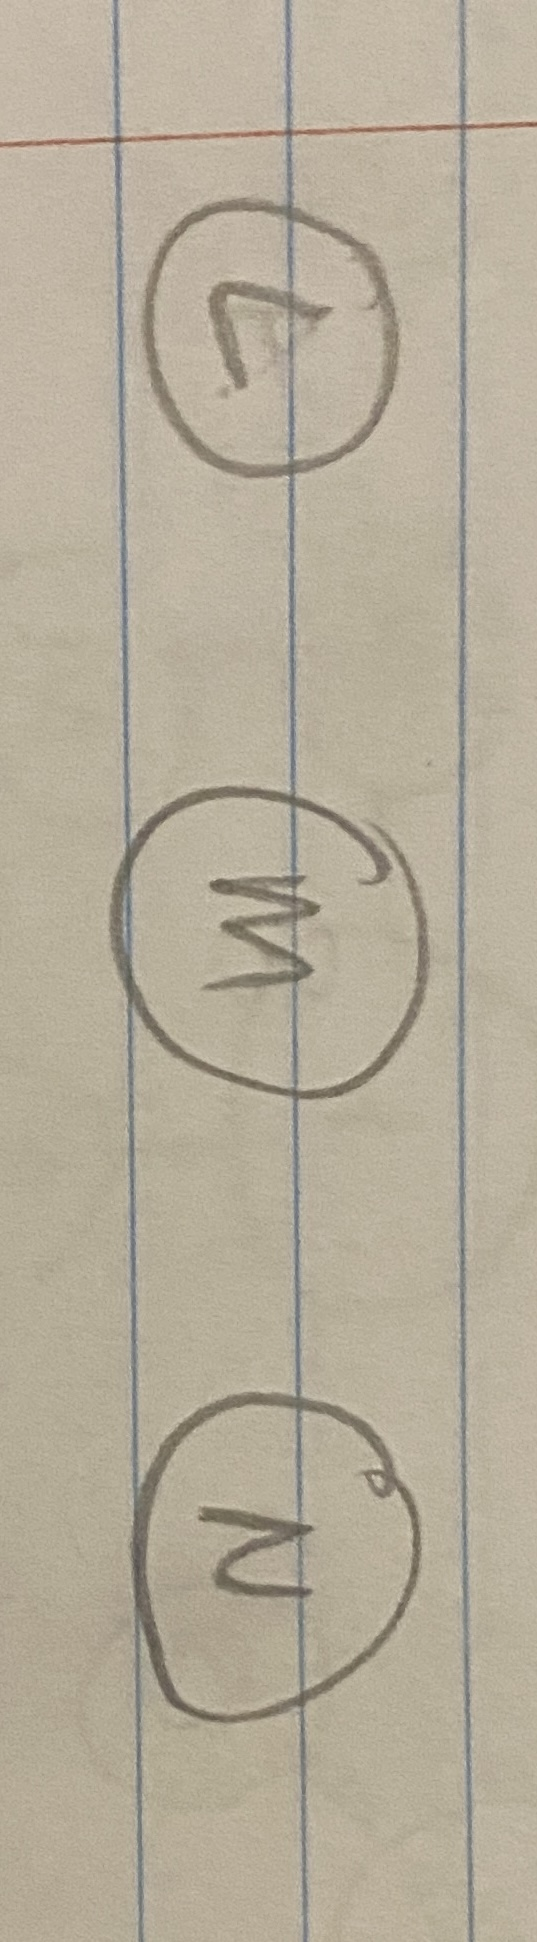
\includegraphics[scale=0.1, angle=90]{1.JPG}
            \item We will remove the minimum node from the Heap (using the delete-min operation) - this is the node L\\
            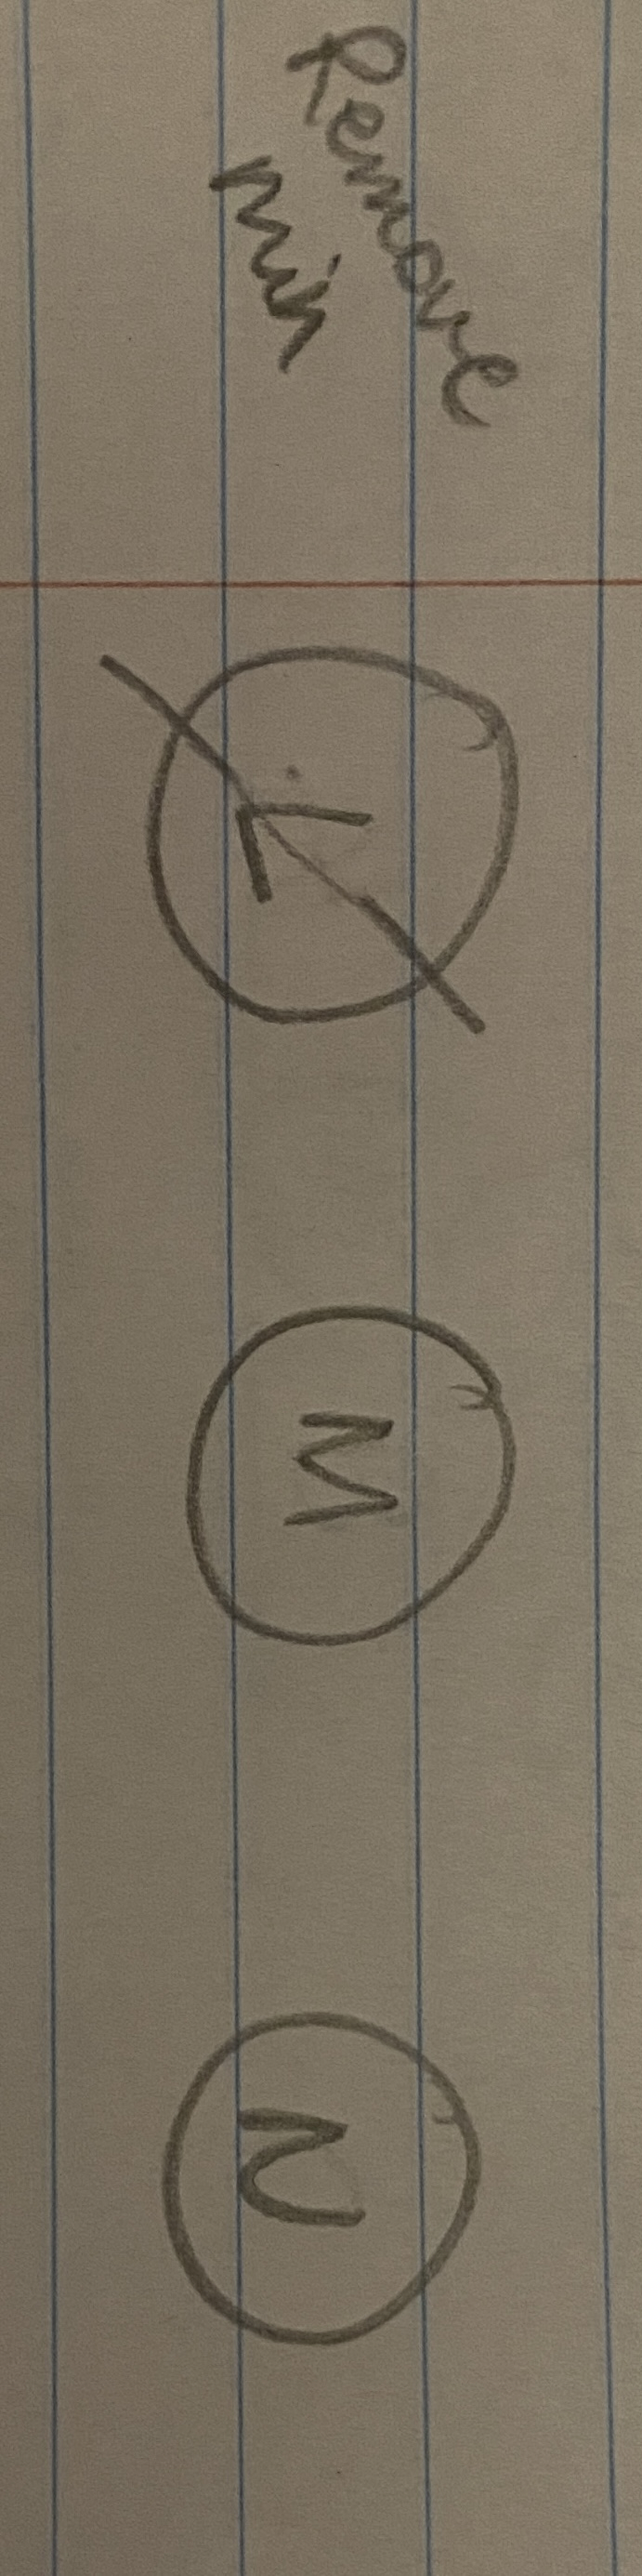
\includegraphics[scale=0.1, angle=90]{2.JPG}
            \item Since the nodes M and N have the same degree of 0, we will consolidate them\\
            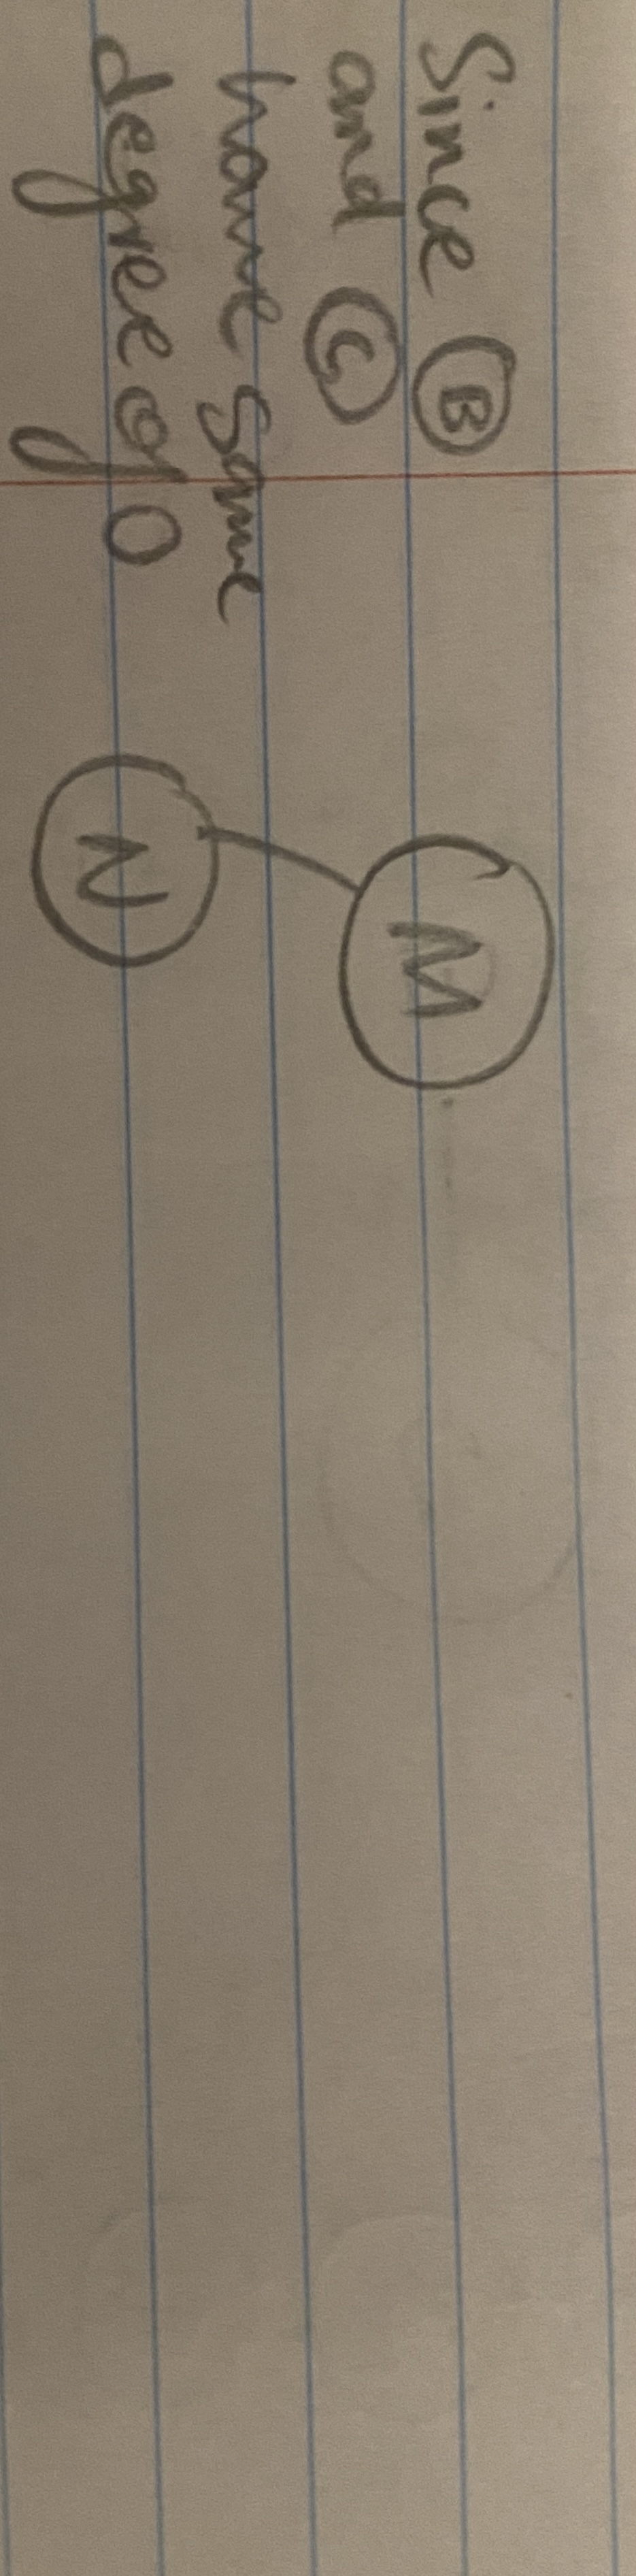
\includegraphics[scale=0.1, angle=90]{3.JPG}
            \item We again add three more nodes. Two of these are nodes smaller than M, and one of them is bigger than M\\
            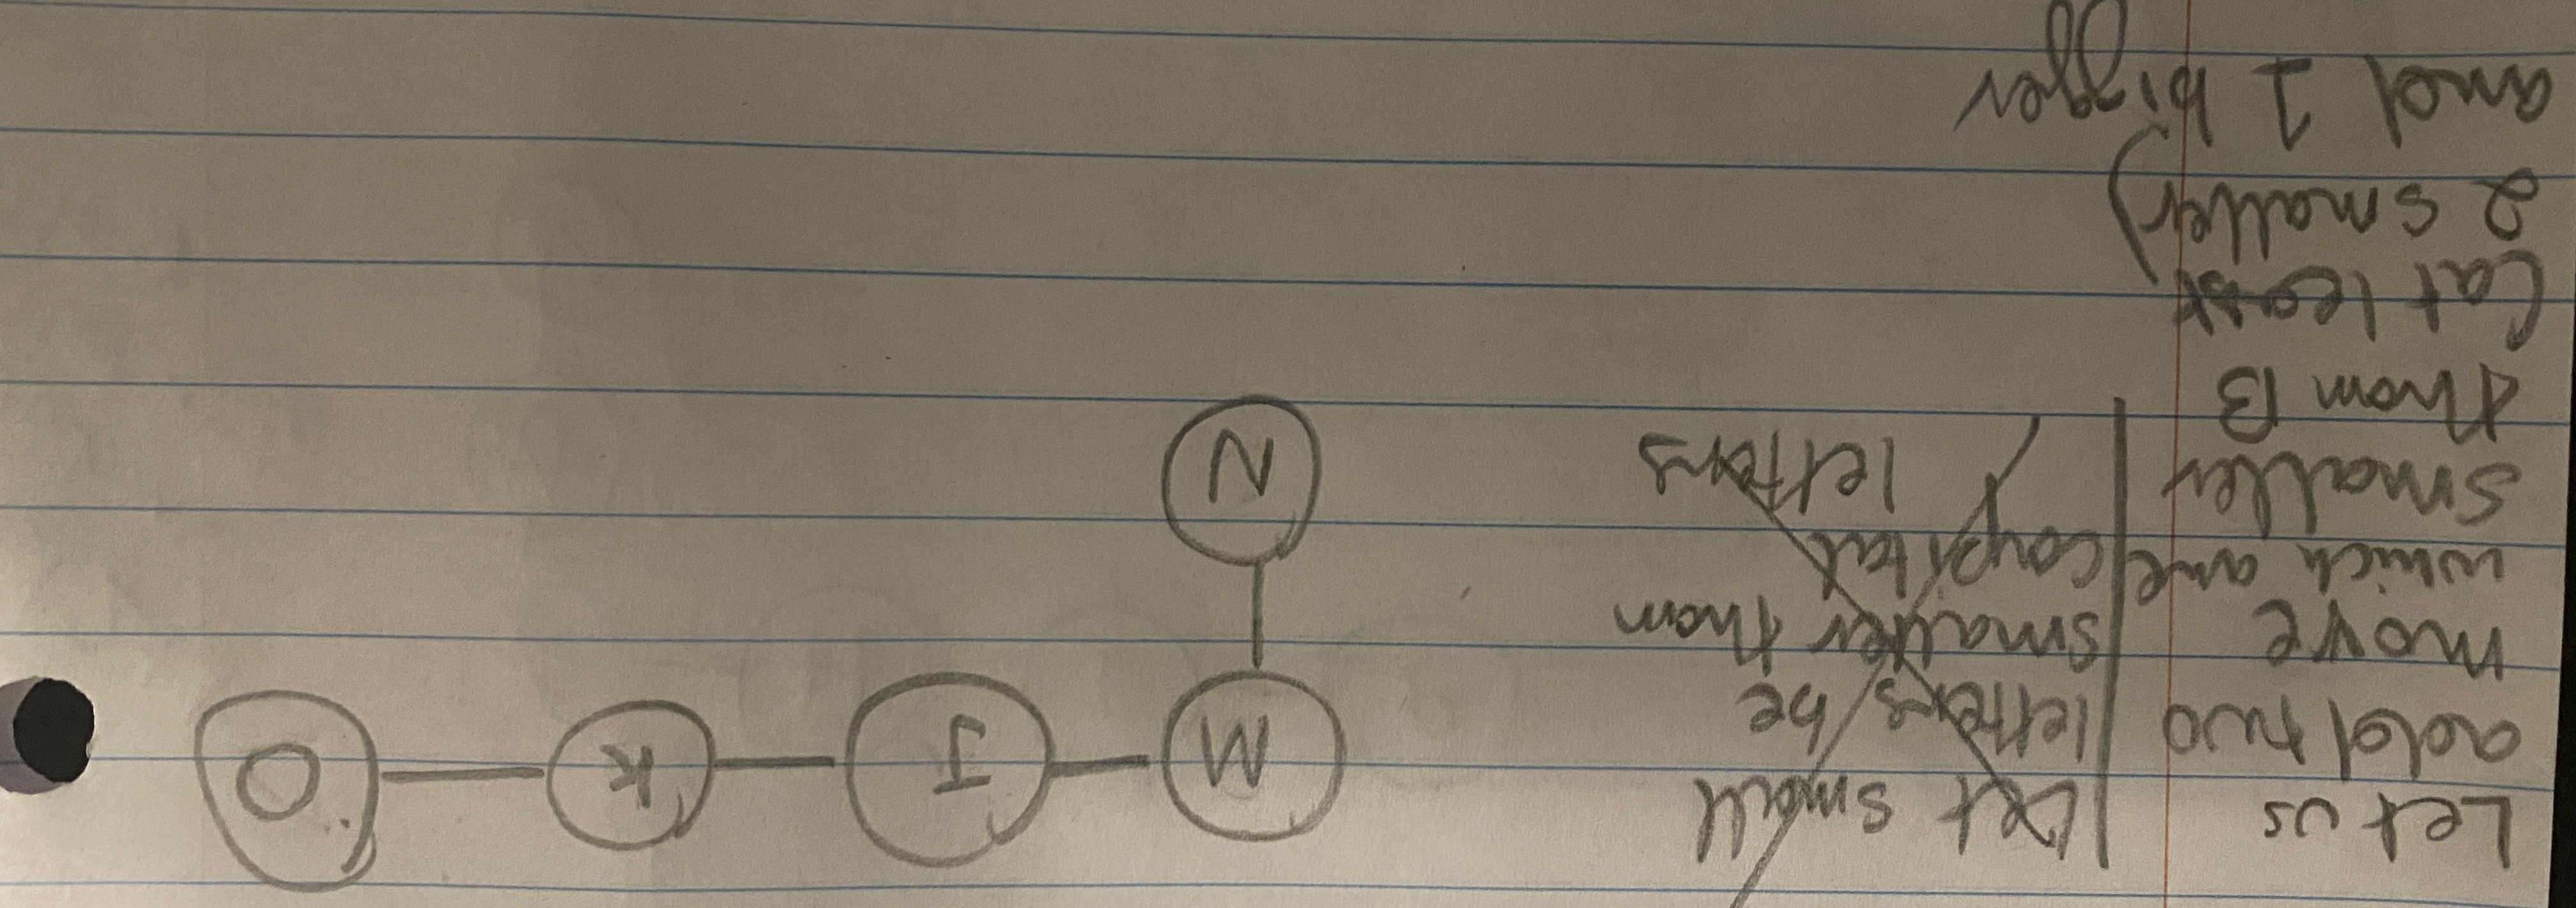
\includegraphics[scale=0.1, angle=180]{4.JPG}
            \item We will remove the minimum node from the Heap (using the delete-min operation) - this is the node J\\
            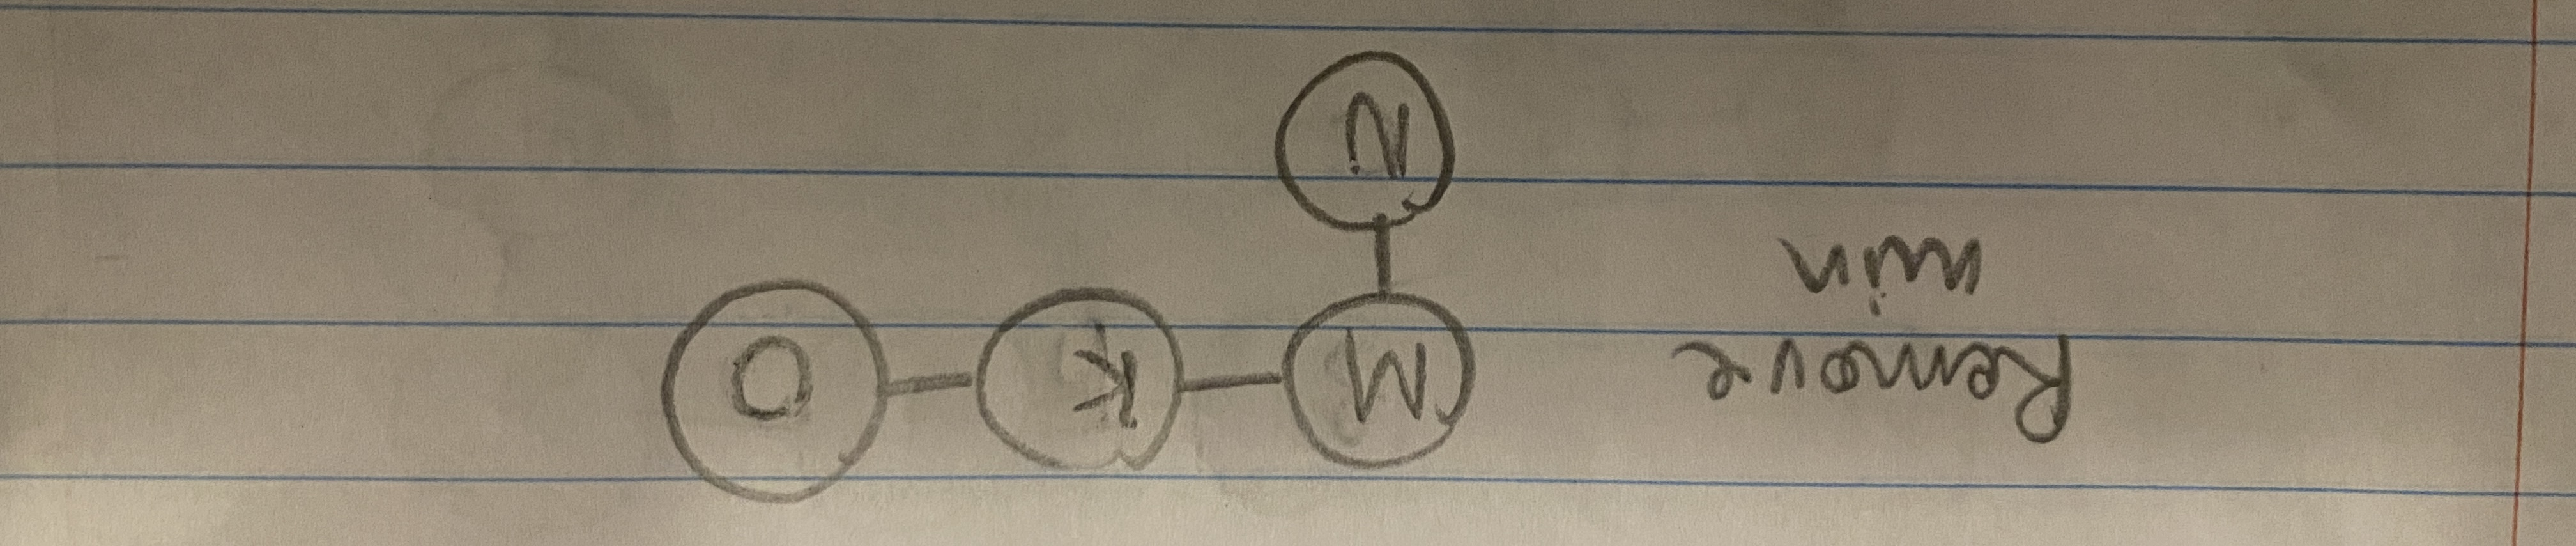
\includegraphics[scale=0.1, angle=180]{5.JPG}
            \item Since the nodes K and O have the same degree of 0, we will consolidate them\\
            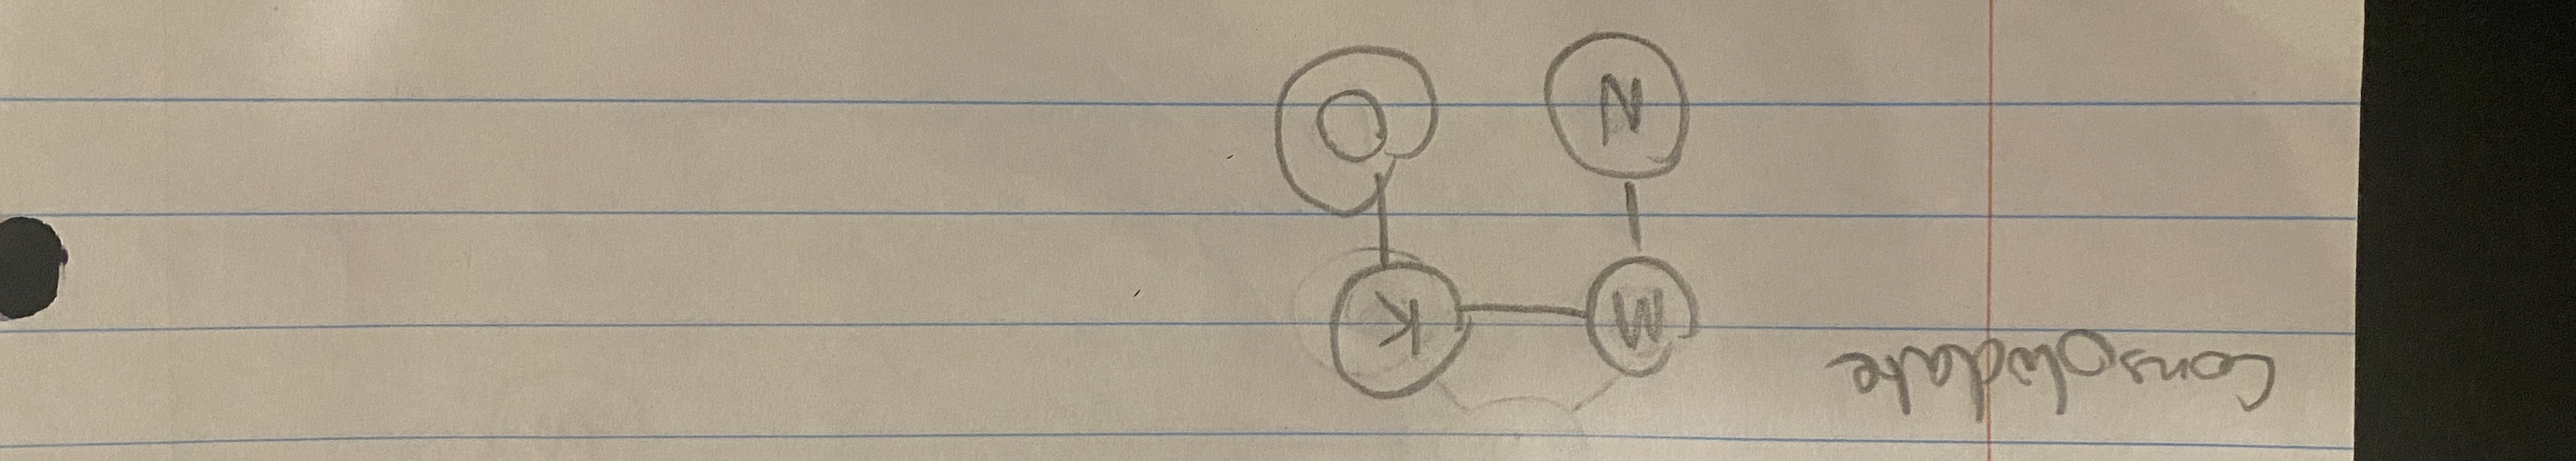
\includegraphics[scale=0.1, angle=180]{6.JPG}
            \item We can further consolidate the structure to make K the root node. This is done because both nodes M and K had the same degree, of 1\\
            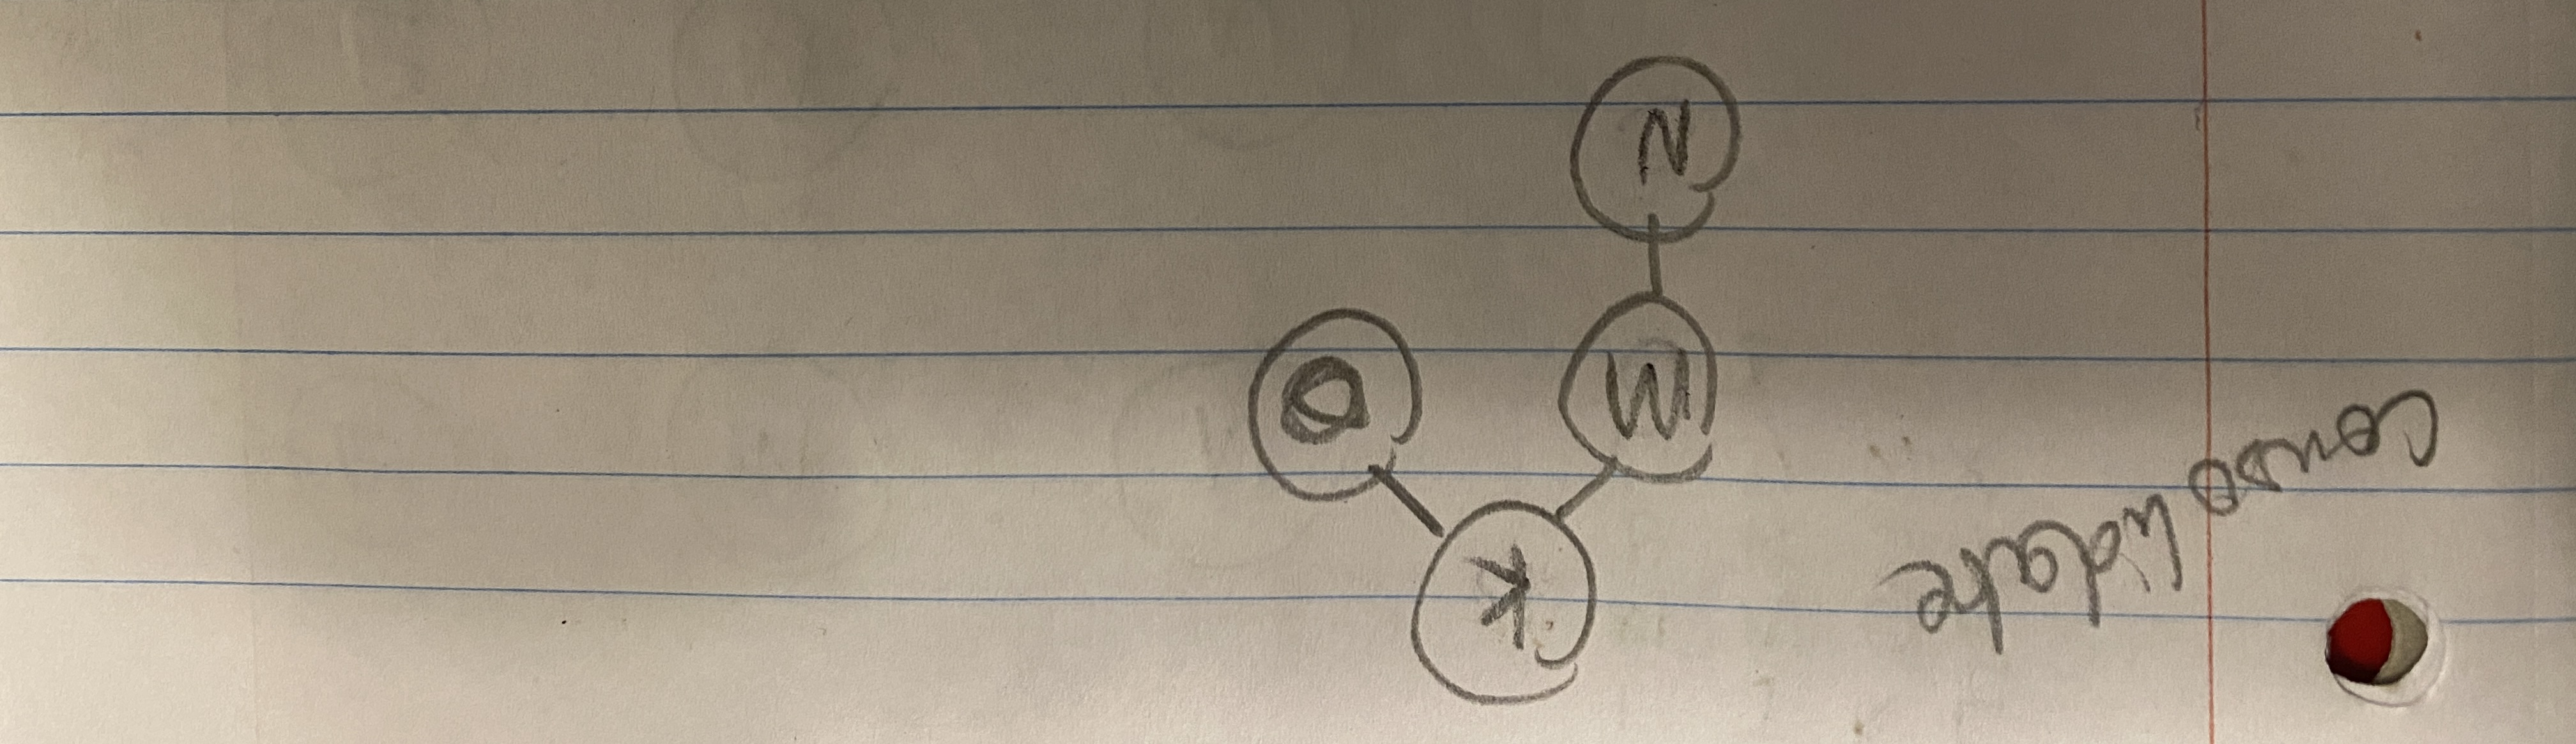
\includegraphics[scale=0.1, angle=180]{7.JPG}
            \item Now we delete O, the single child. Since K has lost a child, it is highlighted (to indicate the same)\\
            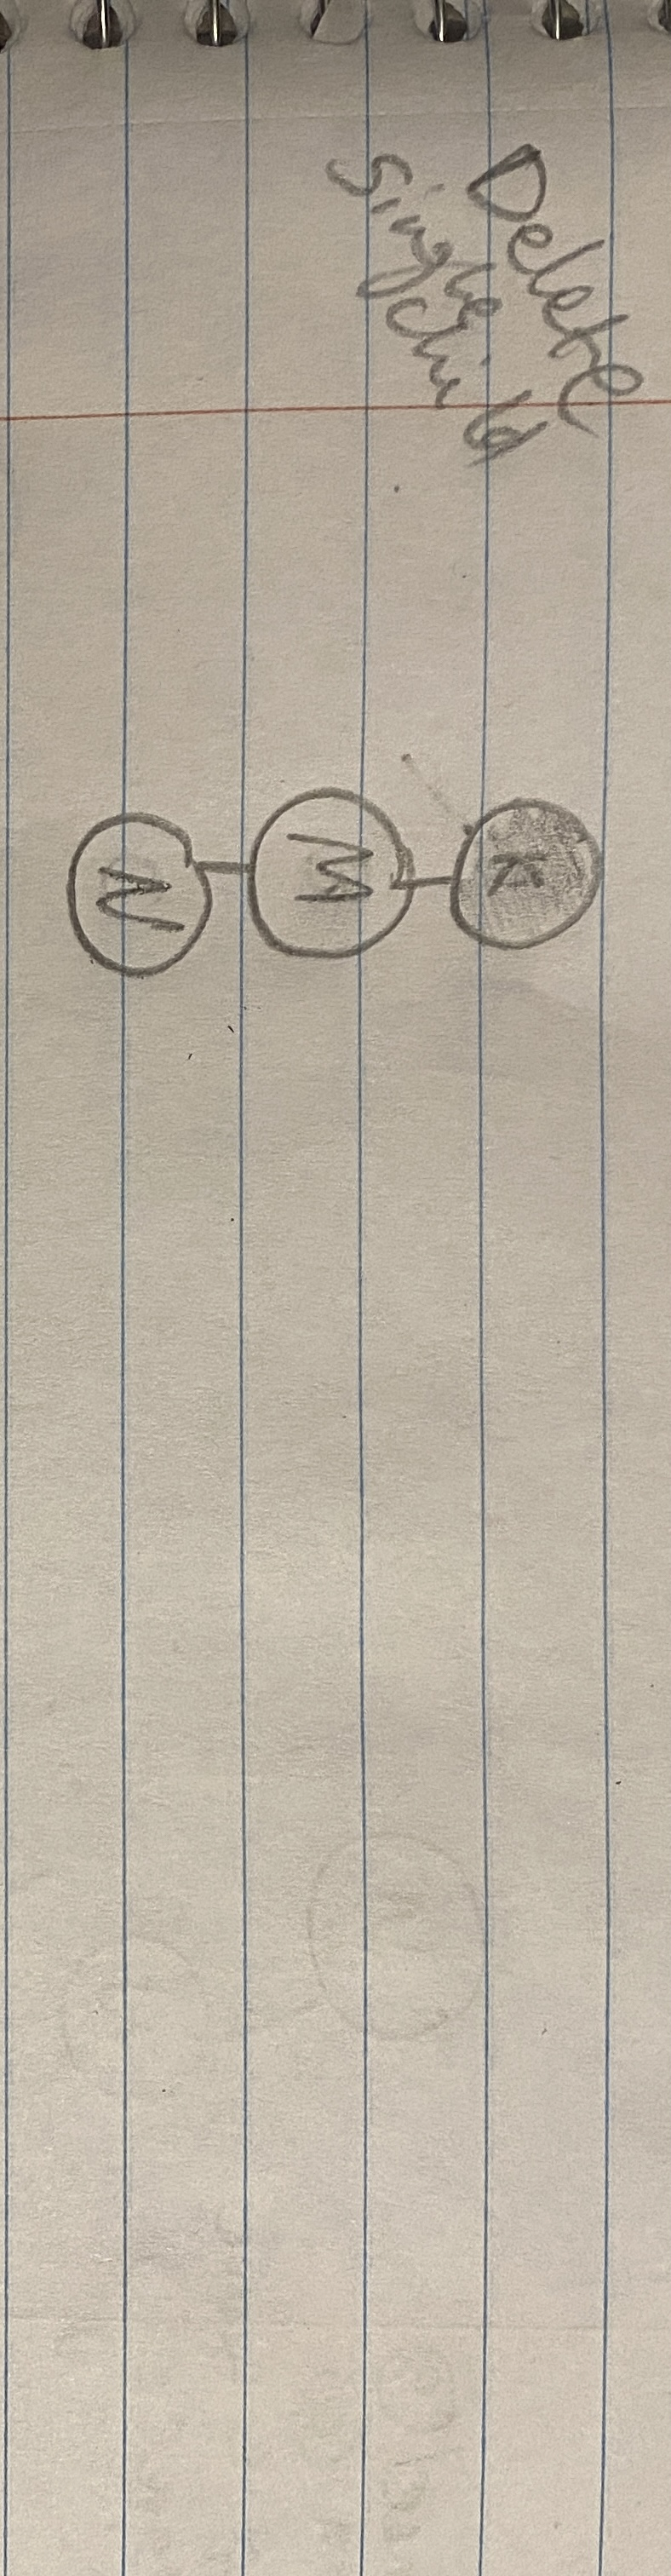
\includegraphics[scale=0.1, angle=90]{8.JPG}
            \item We again add three more nodes. Two of these are nodes smaller than K, and one of them is bigger than K\\
            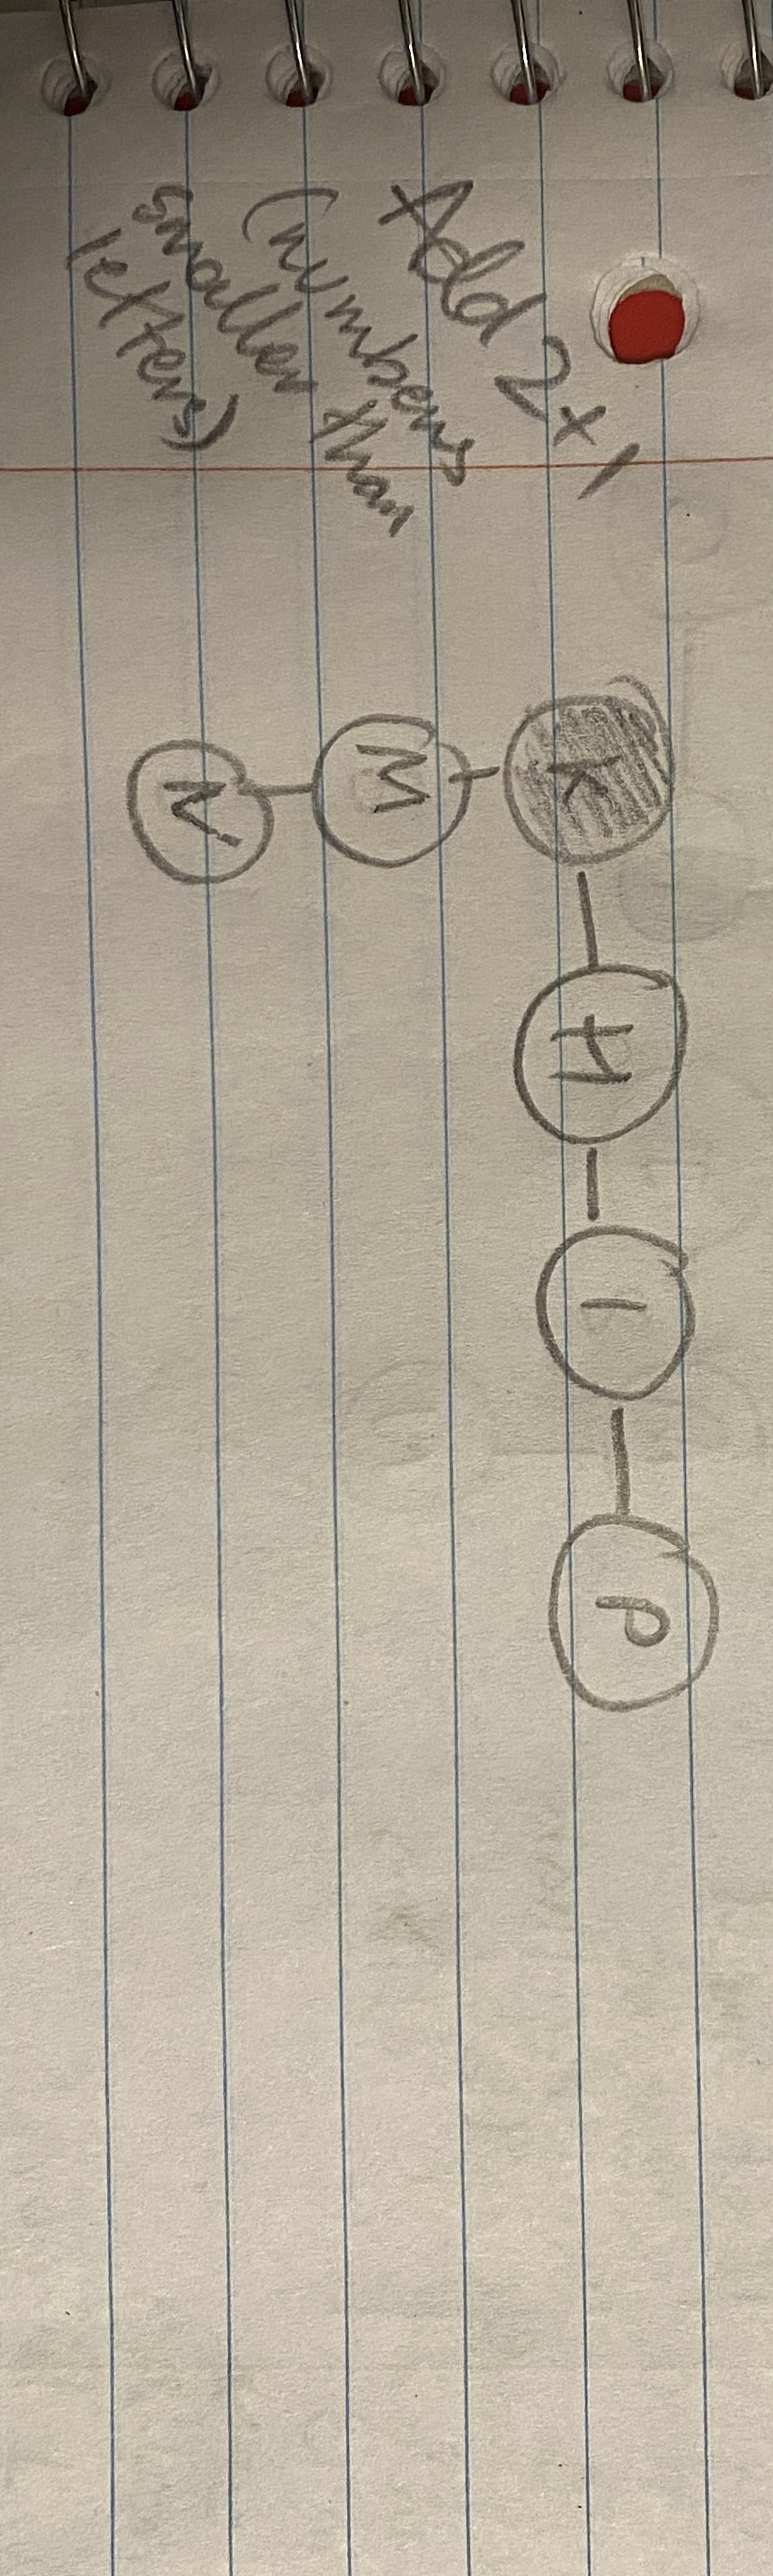
\includegraphics[scale=0.1, angle=90]{9.JPG}
            \item We will remove the minimum node from the Heap (using the delete-min operation) - this is the node H\\
            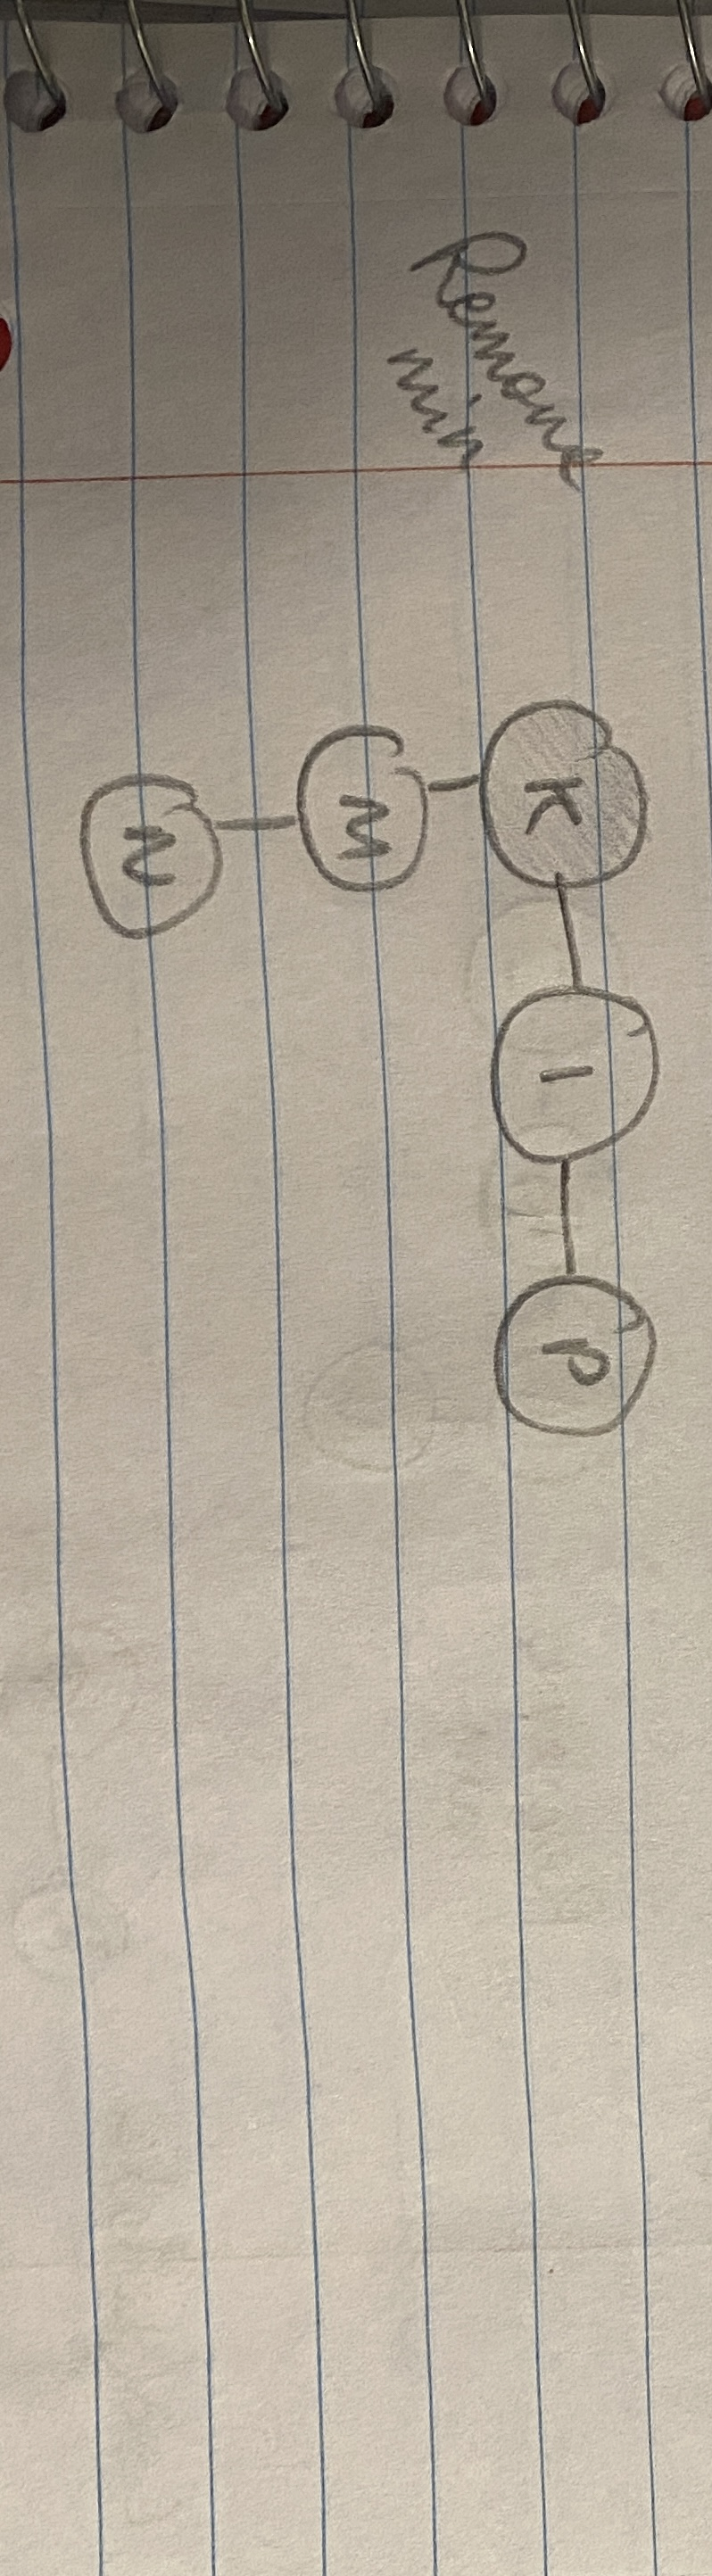
\includegraphics[scale=0.1, angle=90]{10.JPG}
            \item Since the nodes I and P have the same degree of 0, we will consolidate them\\
            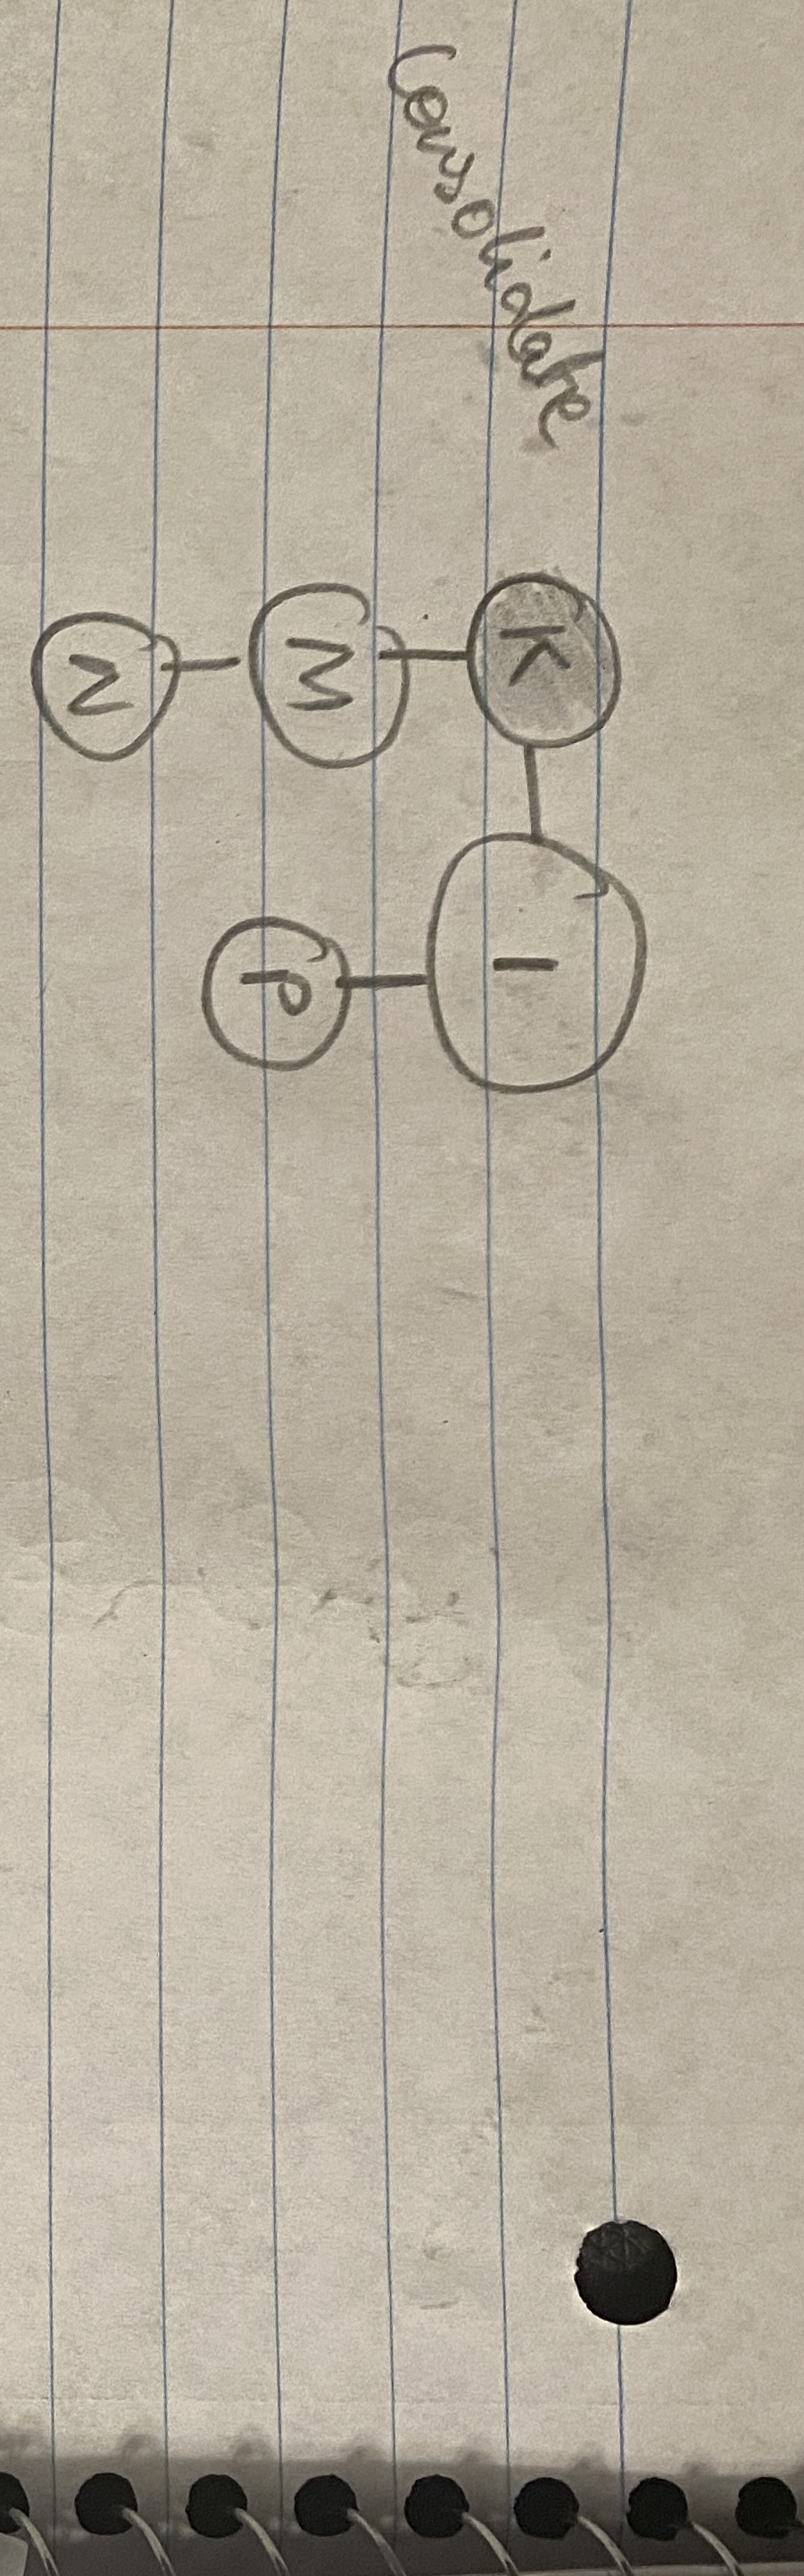
\includegraphics[scale=0.1, angle=90]{11.JPG}
            \item We can further consolidate the structure to make I the root node. This is done because both nodes I and K had the same degree, of 1 (degree is the branching factor)\\
            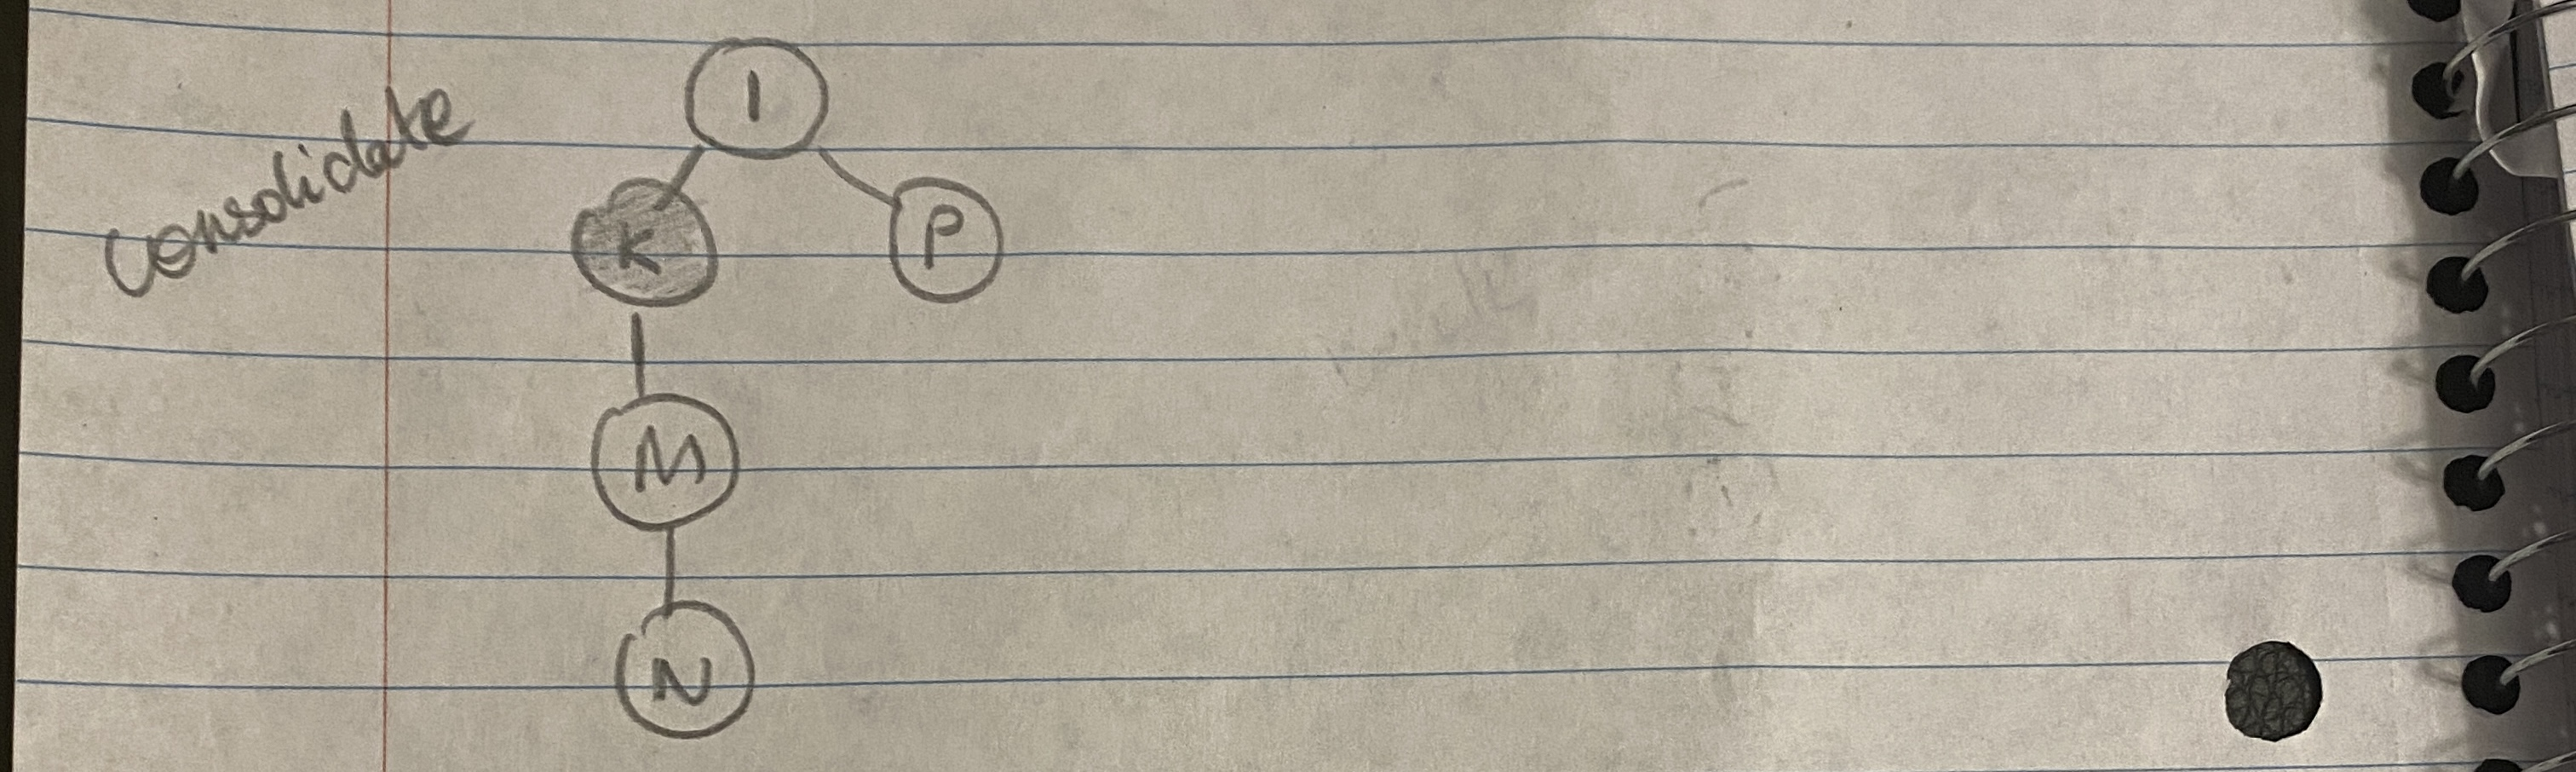
\includegraphics[scale=0.1]{12.JPG}
            \item Now we delete P, the single child. Since I has lost a child, it is highlighted (to indicate the same)\\
            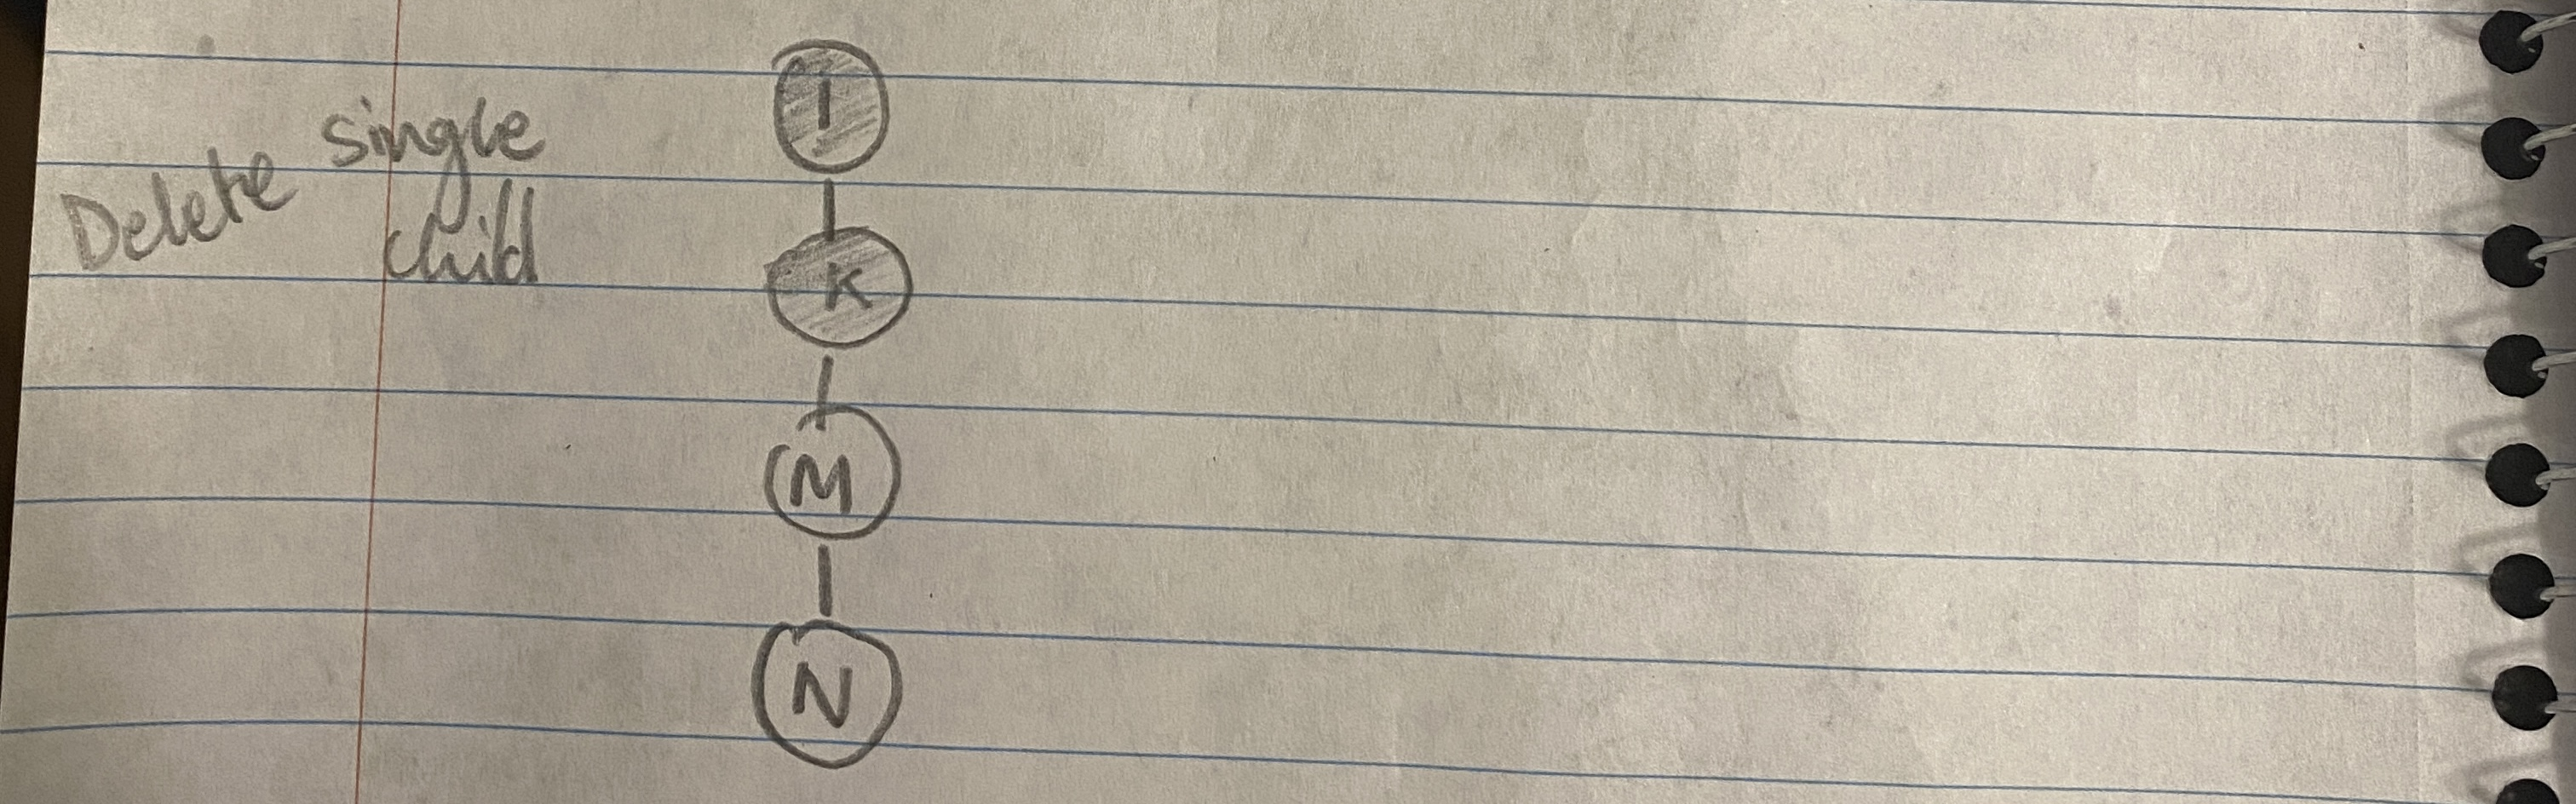
\includegraphics[scale=0.1]{13.JPG}
            \item We again add three more nodes. Two of these are nodes smaller than I, and one of them is bigger than I\\
            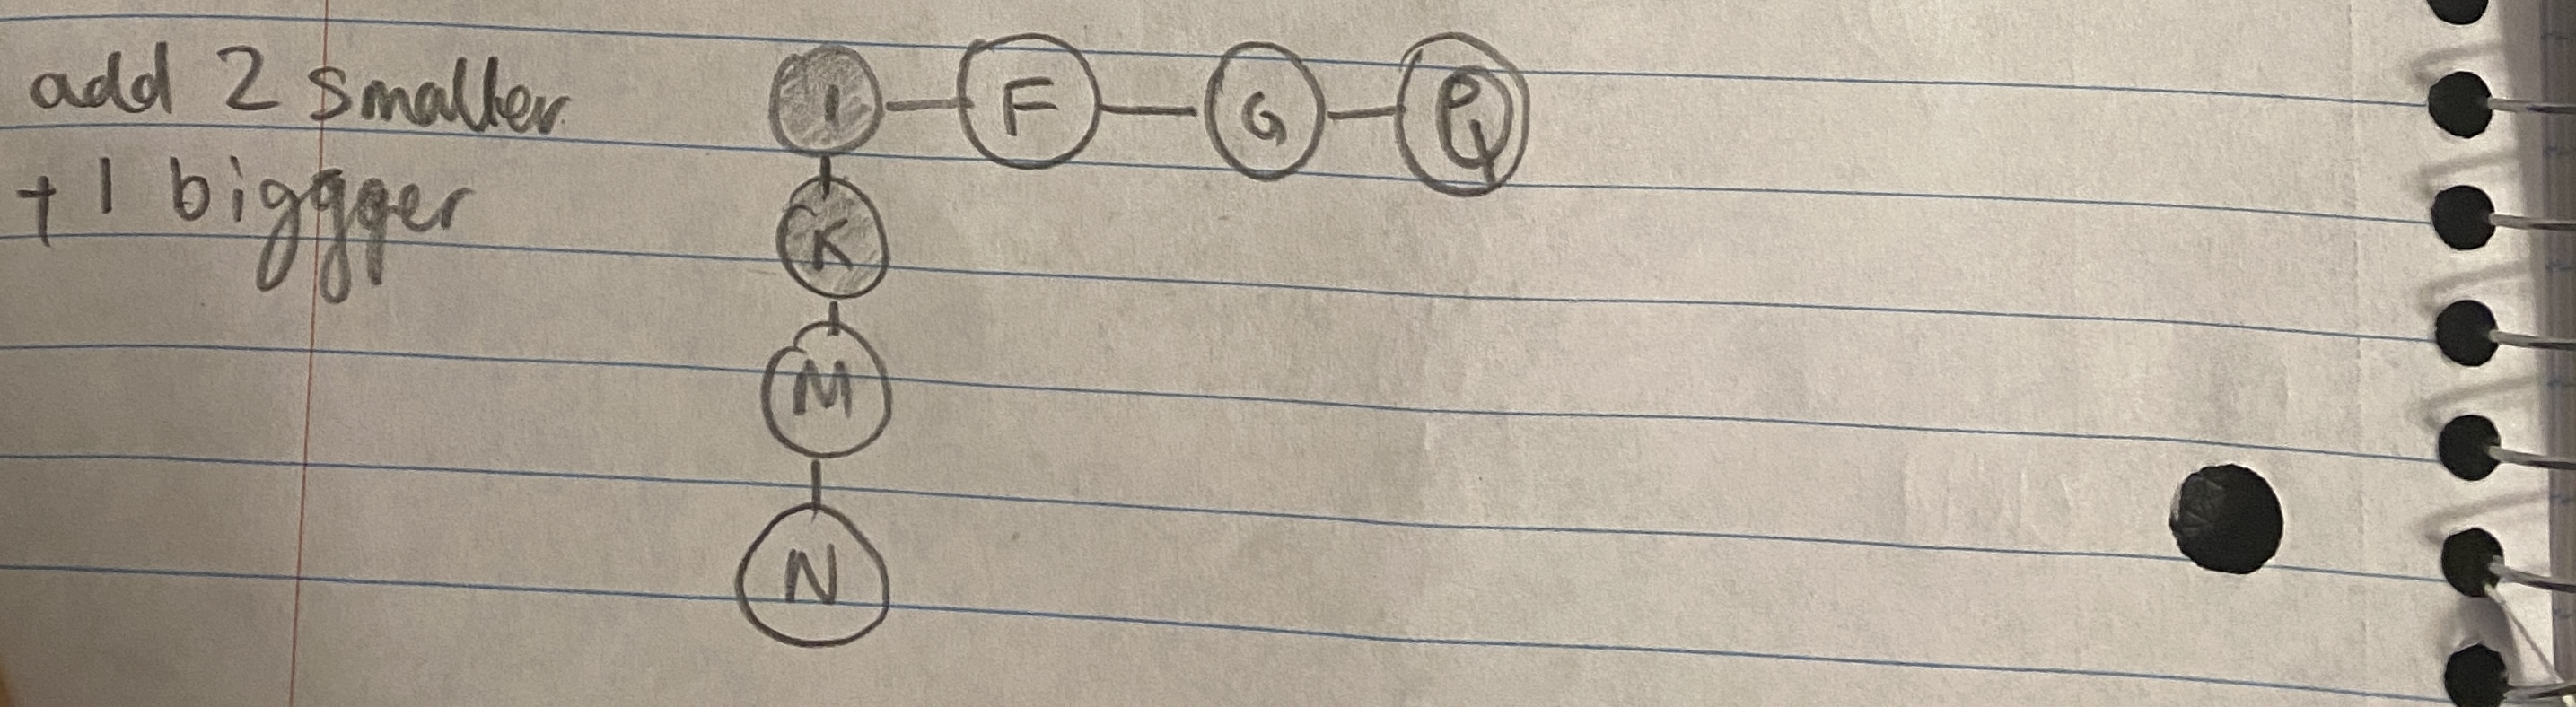
\includegraphics[scale=0.1]{14.JPG}
            \item We will remove the minimum node from the Heap (using the delete-min operation) - this is the node F\\
            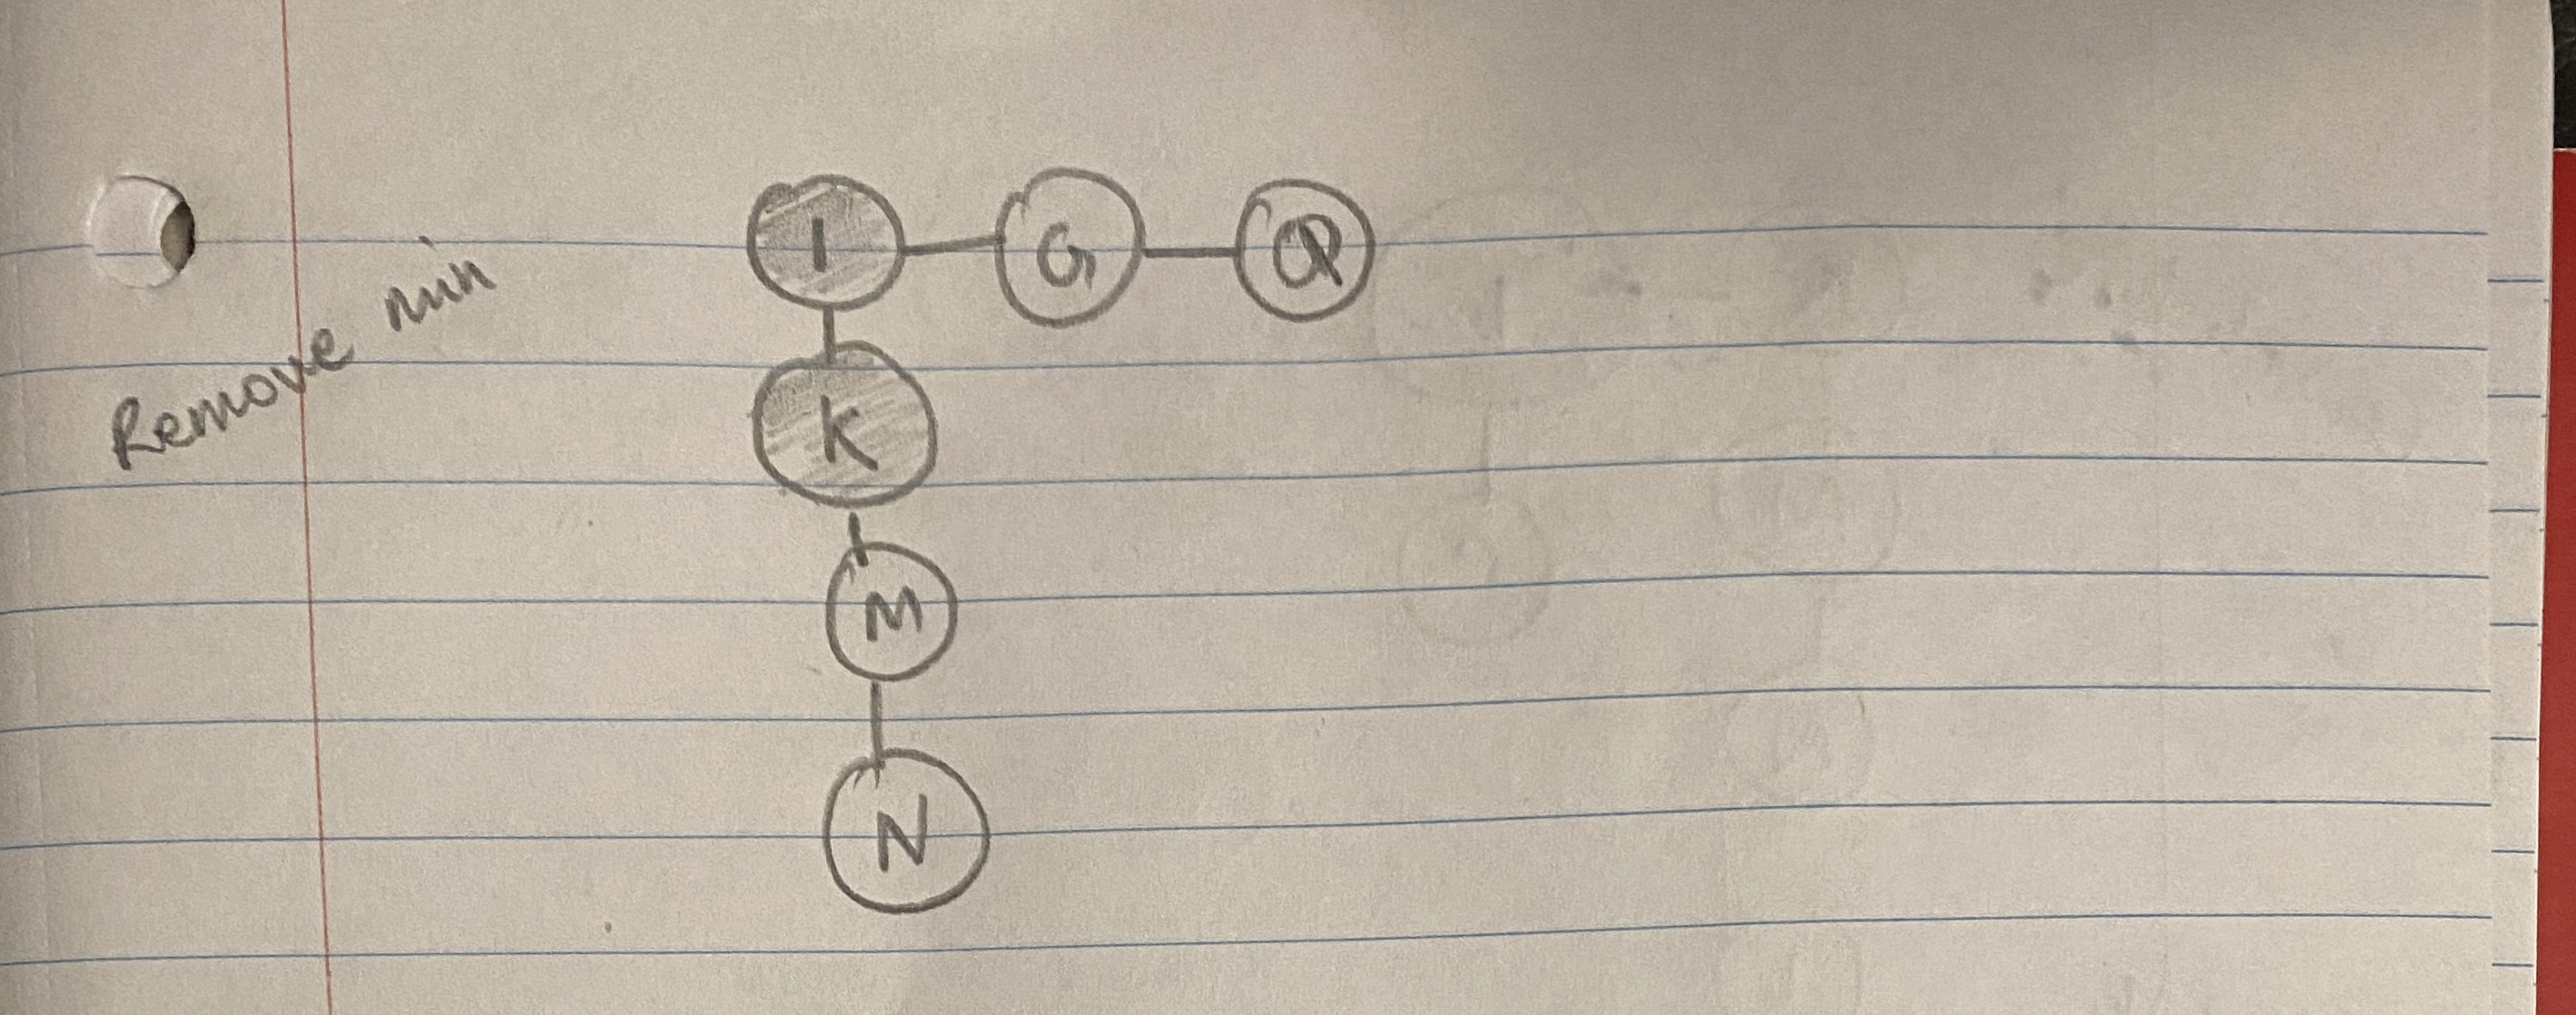
\includegraphics[scale=0.1]{15.JPG}
            \item Since the nodes G and Q have the same degree of 0, we will consolidate them\\
            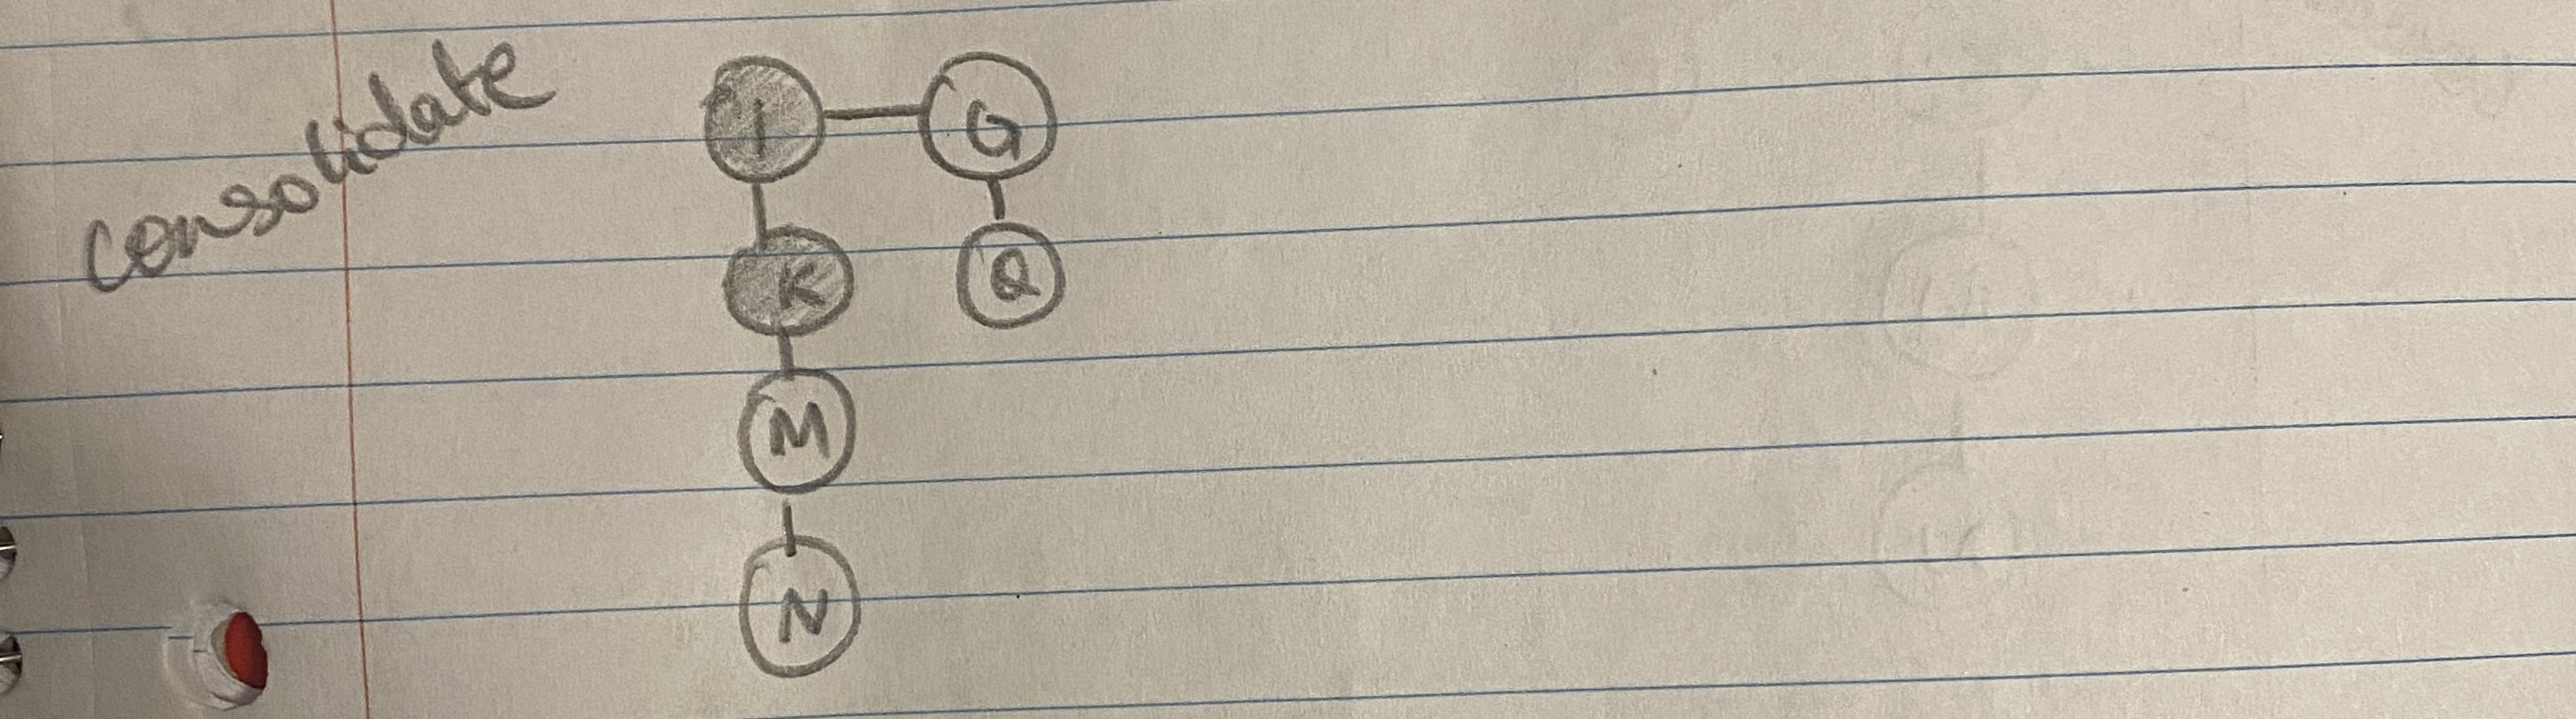
\includegraphics[scale=0.1]{16.JPG}
            \item We can further consolidate the structure to make G the root node. This is done because both nodes I and G had the same degree, of 1 (degree is the branching factor)\\
            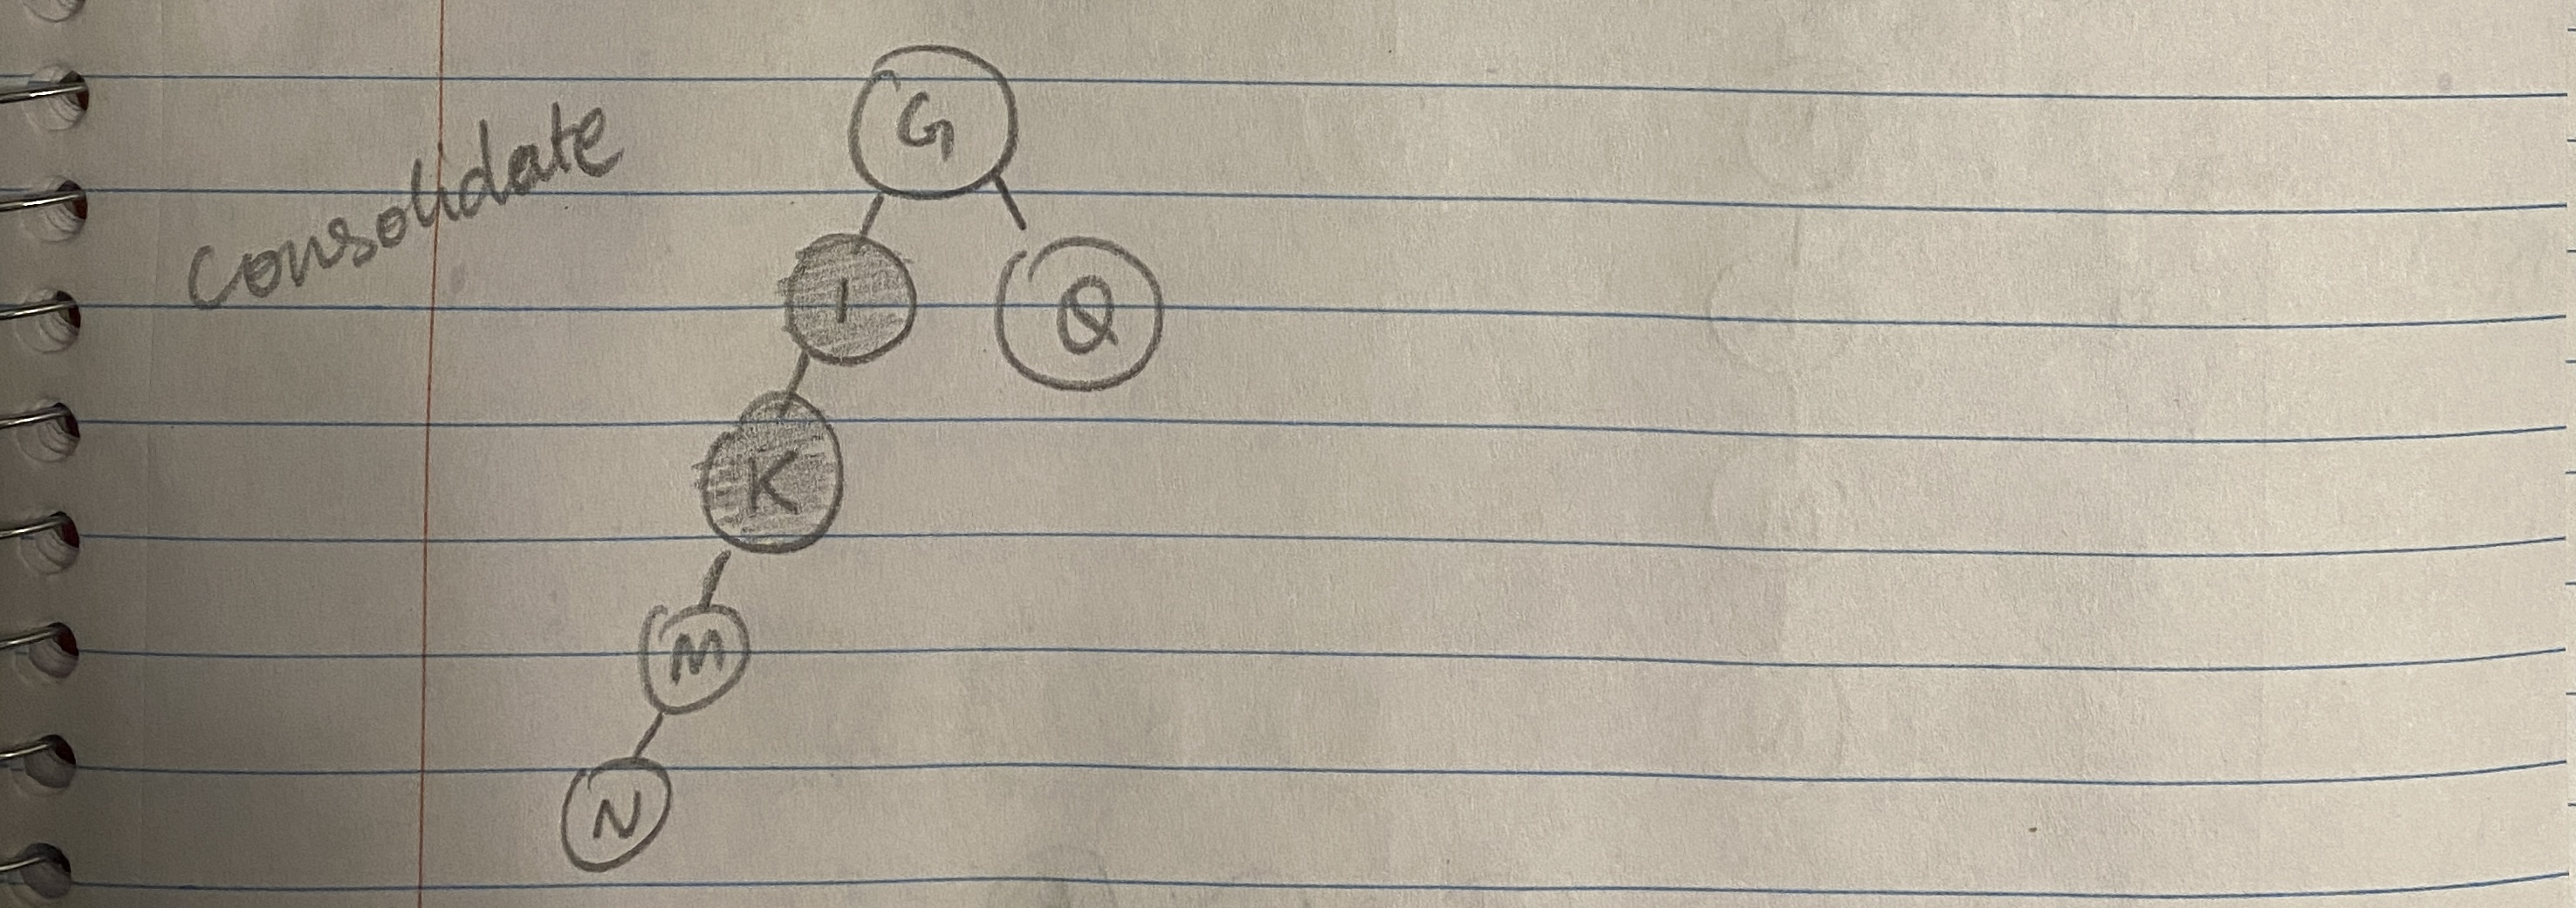
\includegraphics[scale=0.1]{17.JPG}
            \item Now we delete Q, the single child. Since G has lost a child, it is highlighted (to indicate the same)\\
            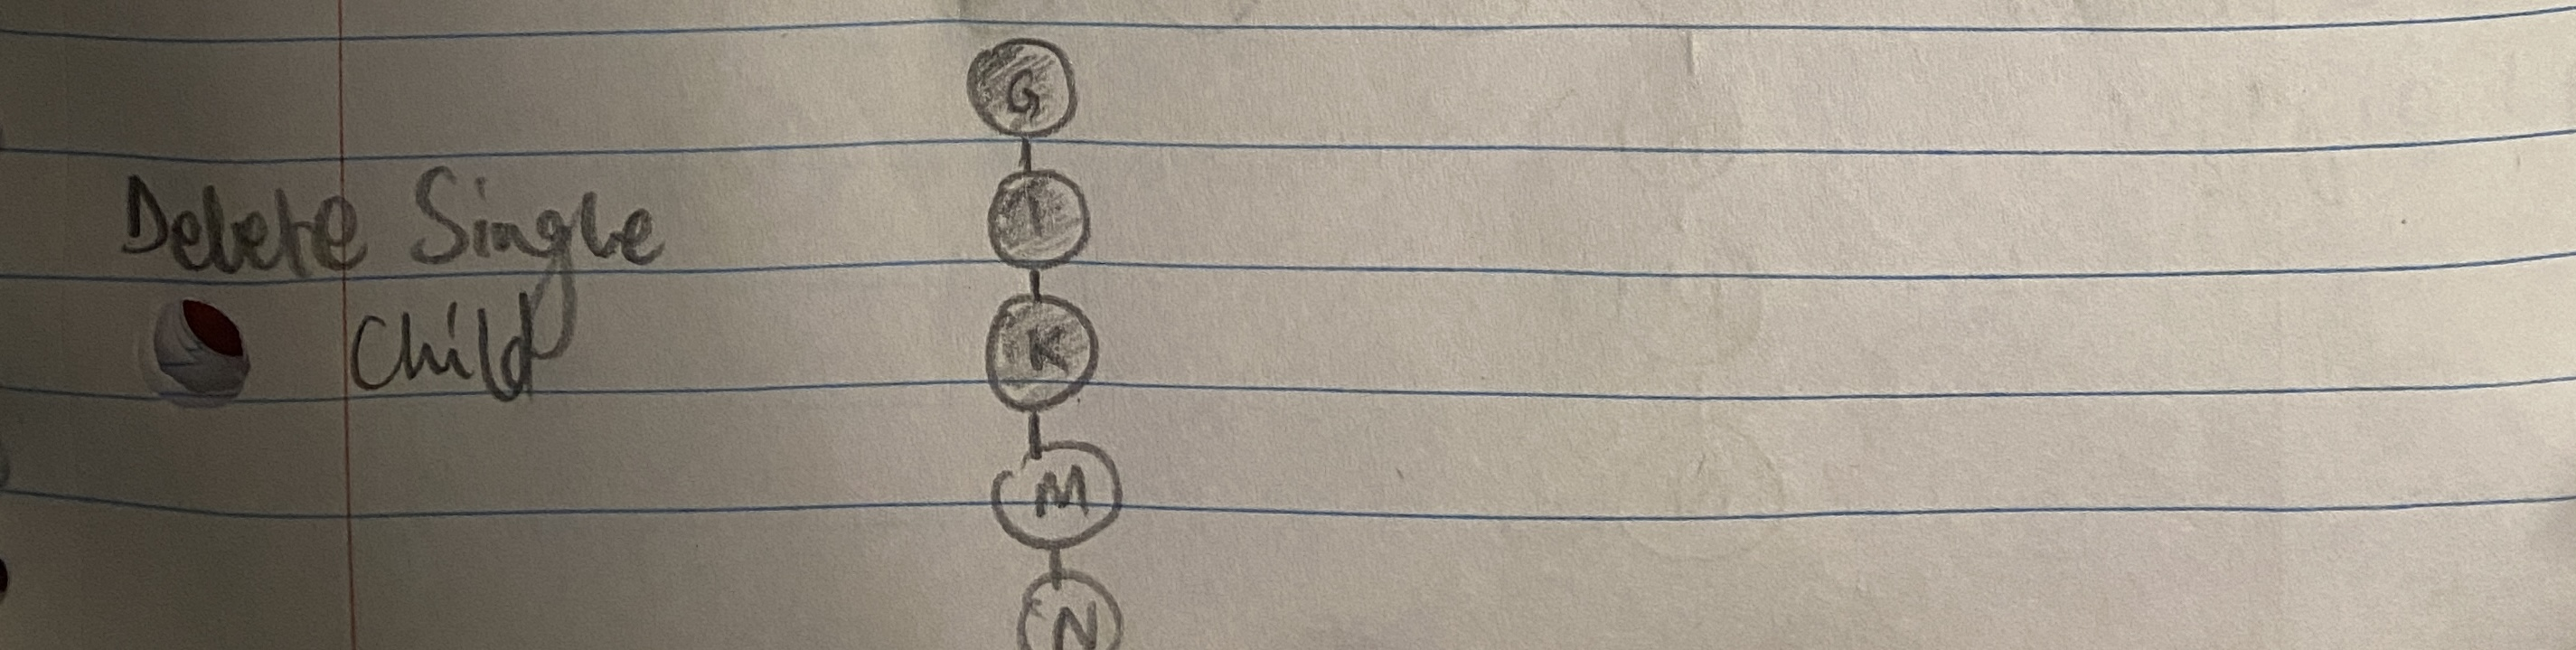
\includegraphics[scale=0.1]{18.JPG}
            
            \item Given the structure of the tree (linear), we notice that if the Fibionacci heap is size n, then its height will be n-1
            
        \end{enumerate}
        \item Argue that in any such heap (not just in your example), at least n-2 of the nodes have lost a child.
        \begin{enumerate}
            \item Let us begin with the analysis of the example from a). In it, we see that there were three occurrences when a subtree had a single node. This was seen in picture ix, xiii, xviii of the example. In the last picture xix, we see that three nodes are marked, indicating that they lost a child. These nodes are G, I, and K. Given that three nodes are marked, and there are a total of 5 vertices in the heap, proving that at least n-2 of the nodes have lost a child.
            \item \textbf{In general}: The statement in the question is true because if a heap has two nodes, we will be required to delete the child node of the root which lies in the subtree containing only one child. 
            \item In the scenario when the root has two subtrees (seen in stages xviii, xiii, and ix), we have been deleting the subtree containing only one node.
            \item Since n-2 or more subtrees will have a single node, the number of nodes that have lost a child will be at minimum n-2.
        \end{enumerate}
    \end{enumerate}
    \textit{Reminder: } CascadingCut does not mark a root when it loses a child.
\pagebreak

\item Problem 2. FH ExtractMin Worst Case.\\
Modify the Fibonacci Heap so that the worst-case time for ExtractMin is O(lg n), rather than O(n). All the FH operations should still have the same amortized time bounds. To accomplish this, you may need to increase the asymptotic worst-case time for some of the other FH operations, which ones?

\textit{Hint: }keep track of t(H), and don't let it get larger than some constant times D(n).
\begin{enumerate}
    \item We will modify the Fibonacci Heap in order to maintain a log of t(H). This would involve adding the following snippet of code after each time the method FH-alter is called.
    \item If z(D(n)+1) $\leq$ t(H):\\
    Consolidate(H)
    \item For some constant e, the real time cost of this operation (consolidating) is at max e(t(H)+D(n)+1)
    \item Let us call the heap that is formed due to this call H'. This heap (H') has $t(H') \leq D(n) + 1$.
    \item Based on the above inequality, the change in function will have value at maximum of -0.5E(H)
    \item Using this, we can calculate the amortized cost of the consolidate operation as: e(t(H) + D(n) + 1) + e(-0.5t(H))\\
    
    This is equal to the actual cost + the change function
    \item The value of the above will always be less than or equal to 0. Due to this understanding, the cost of any of the operations will not exceed O(1).
    \item Further, this implies that t(H) is constrained to the O(log n), and this will be its worst case time. Although, operations such as union and insert will be O(1) but in the worst case will have O(log n).
\end{enumerate}
\pagebreak

\item Problem 3. Exercise 25.2-9 (page 700).\\
On computing transitive closure. (\textit{Hint: }you may use the result from CS-253 or Section 22.5, that we can compute the strongly connected components of a digraph in O(V+E) time. Also, the resulting kernel or component graph (page 617) is a DAG.)


Exercise 25.2-9 (page 700):\\
Suppose that we can compute the transitive closure of a directed acyclic graph in ... time, where f is a monotonically increasing function of ... . Show that the time to compute the transitive closure G* = ... of a general directed graph G = ... is then ... .

\begin{enumerate}
    \item to compute the transitive closure of the general directed graph, we should begin by computing the strongly connected components and analyse its component graph. The latter will be acyclic and I expect it cannot have as more vertices and edges than the original graph.
    \item I believe the transitive closure algorithm will be worthwhile performing on the graph, given the graph's acyclic nature. 
    \item Based on this, we use the transitive closure's component graph result to analyse every edge. For each of these edges, another one is added which leads us from $S_1$ to $S_2$. Performing this series of operations is expected to take time equal to O(C+E*)
    \item Using this, to perform the entire sequence of repetitive operations, I expect the time to compond and increase. Based on my calculations, the total time will be at maximum f(|V|, |E|) + O(V+E). Please assume the long dashes are vertical bars. I am trying to represent the absolute value of V and E.
\end{enumerate}
\pagebreak

\item Problem 4. Exercise 25.3-6 (page 705).\\
On Professor Michener's variant of Johnson's algorithm (two parts).
\begin{enumerate}
    \item The original version of Johnson's algorithm:
    \item You add a new vertex S, which is not part of the original graph
    \item You add edges from S to all the original vertices (all these edges have length 0)
    \item For every vertex v: h(v) = delta (s,v)
    \begin{enumerate}
        \item h(v) is set to be the distance from S to v in this augmented graph.
        \item \^w for a given edge (u, v) is the original weight from u to v. Given by $\^w(u,v) = w(u\|v) + h(u)-h(v)$
        \item This is argued to be atleast 0 $(\geq 0)$ by the triangle inequality
        \item Please see the picture below to refer to Johnson's algorithm\\ 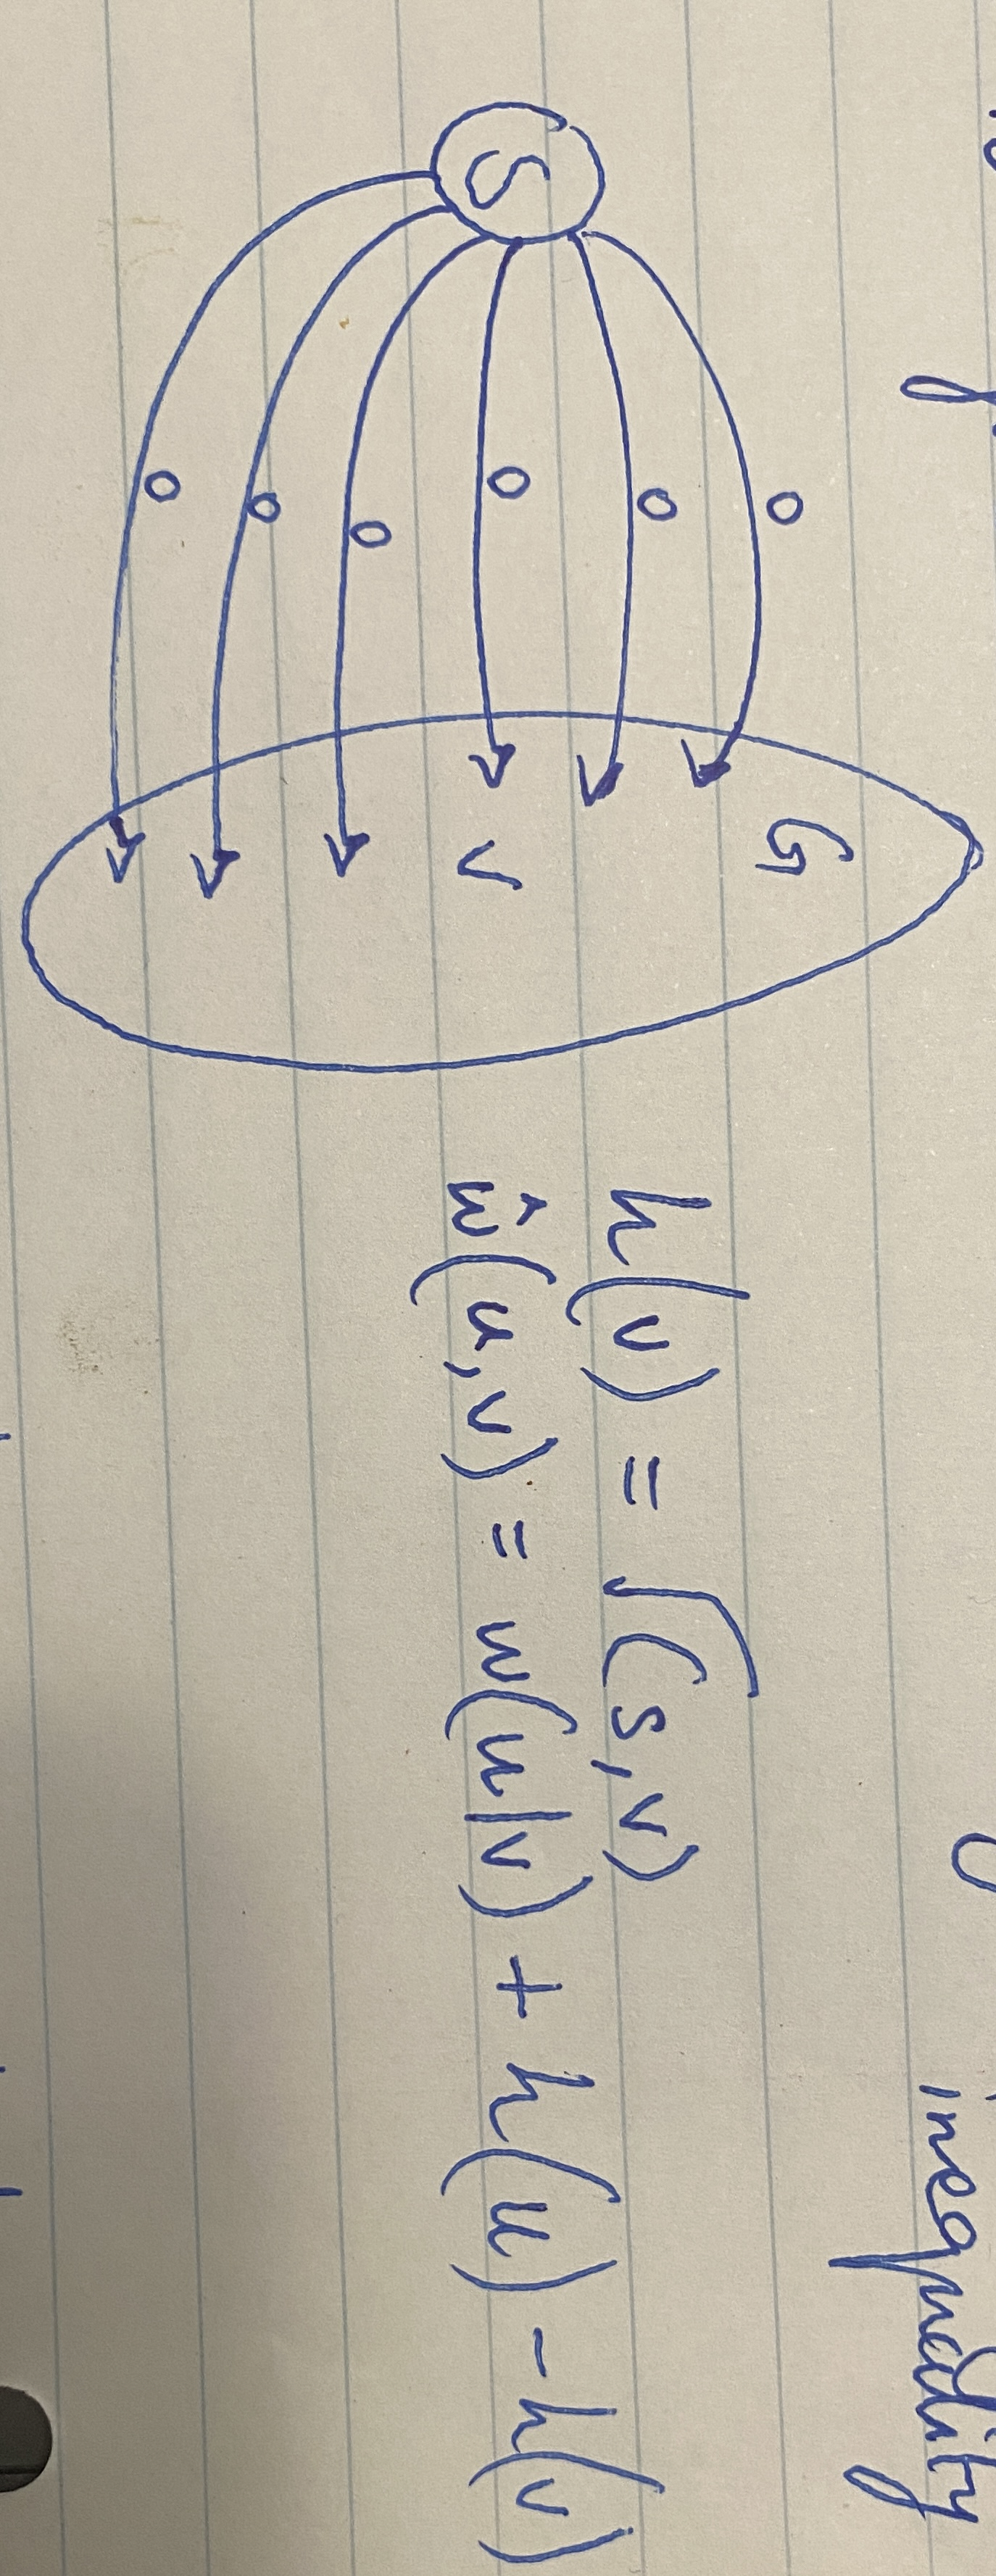
\includegraphics[scale=0.1, angle=90]{IMG_8537.JPG}
    \end{enumerate}
\end{enumerate}
\begin{enumerate}
    \item Prof. Michener's proposal is the same thing but instead use an existing vertex S.
    \item Considering whether it will work signifies looking at two slides:
    \begin{enumerate}
        \item If some vertices are not reachable from S, it does not work
        \item The above is true because if they are not reachable, then those distances must be infinite
        \item If delta(s,u) = +inf or delta(s,v) = +inf or both of these, then:
        \item we do not have a sensible way to define h(u) - h(v) anymore. Since we are adding and subtracting infinity (which is undefined) in h(u) - h(v), then w is also not defined.
        \item An example of a graph G where S (a vertex in G) does not reach all or some of the other vertices
    \end{enumerate}
    \item Alternatively, if you can reach all other vertices from S. So that means that delta(s,v) is never infinity (delta(s,v) $<$ inf)\\
    Then it can be shown that it does work (this is shown using the triangle-inequality/argument)
    \begin{enumerate}
        \item Triangle inequality:
        \item If you have a shortest path from s to u, and another shortest path from s to v. And an edge directly from u to v with w(u,v)
        \item Since the s to u and s to v are the shortest paths. It means that the direct path from u to v + the other path must be longer (eg: delta(s,u) + w(u,v) is longer than delta(s,v)). See image below\\ 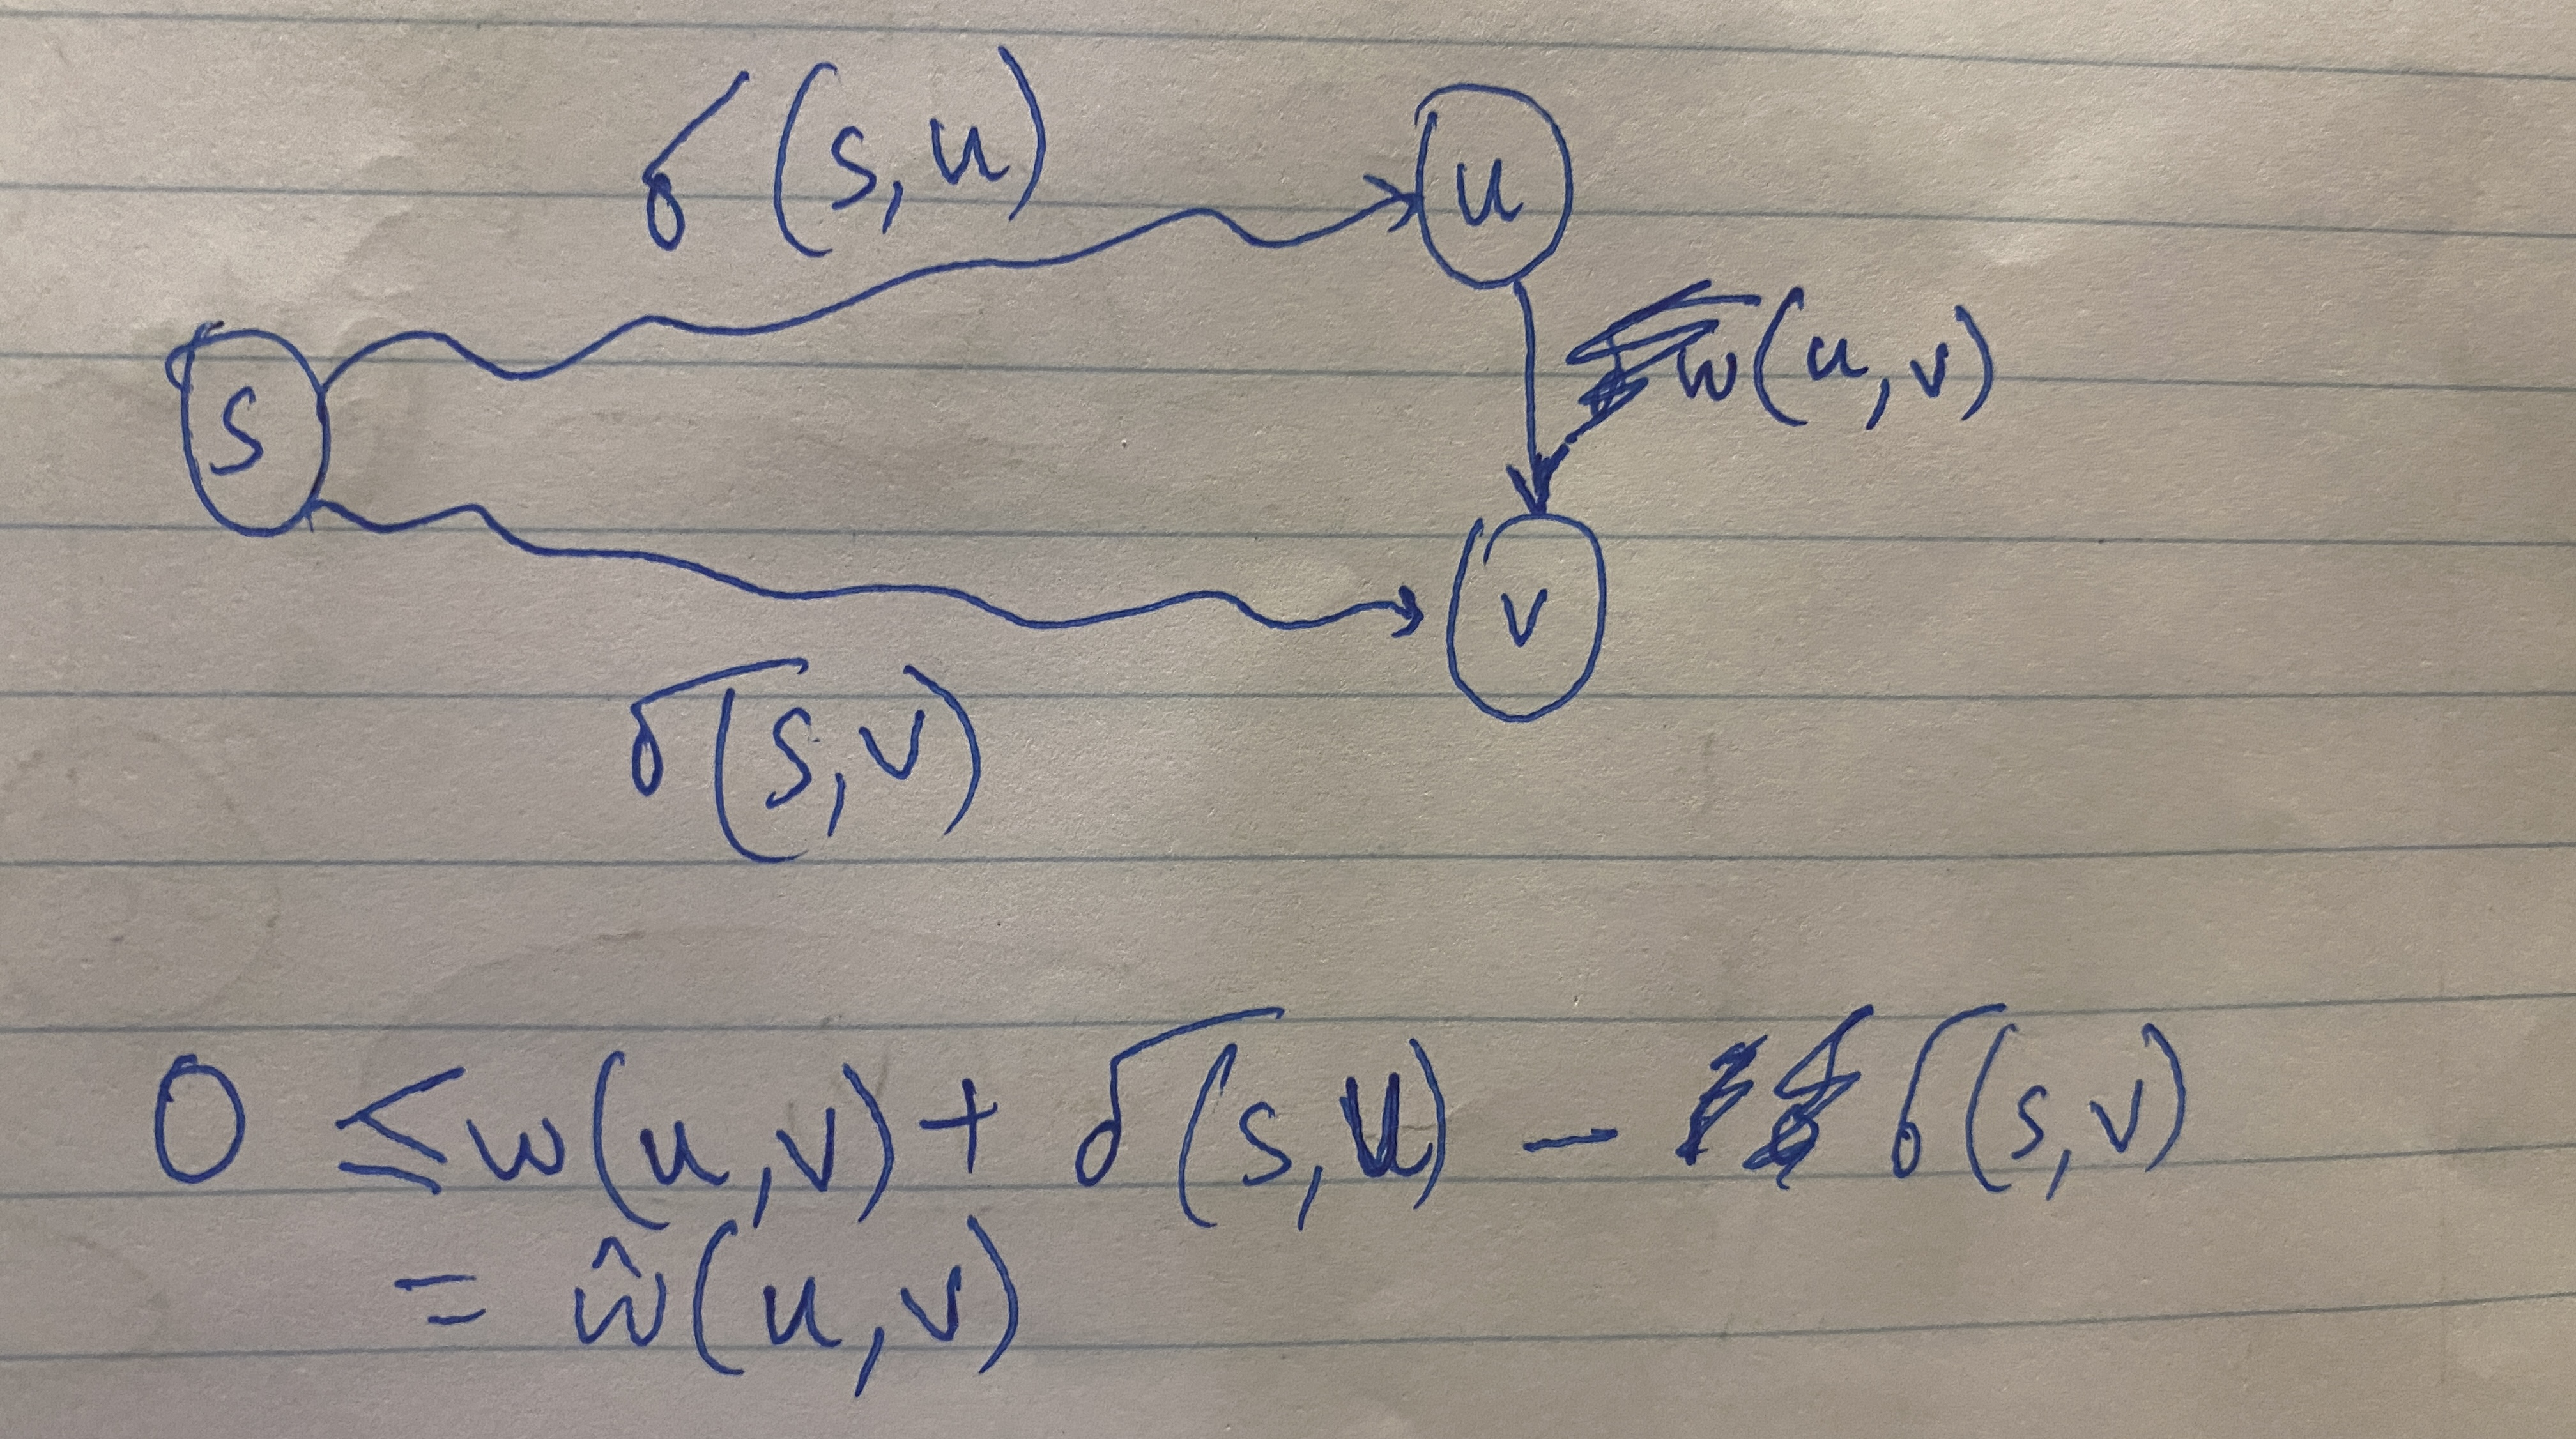
\includegraphics[scale=0.1]{IMG_8541.JPG}
    \end{enumerate}
    \item It is worthwhile to see that this argument still works without making S a separate vertex
    \item In the directed graph seen below, the Professor's claim will not be valid because if A is the Starting state, there is no way to reach back to A. Using the Bellman Ford Algorithm, we will see that h(A) is infinity since there is no way to reach from B (to A) and hence, when we start at B, we will not have a value for \^w(B, A). 
    \\ 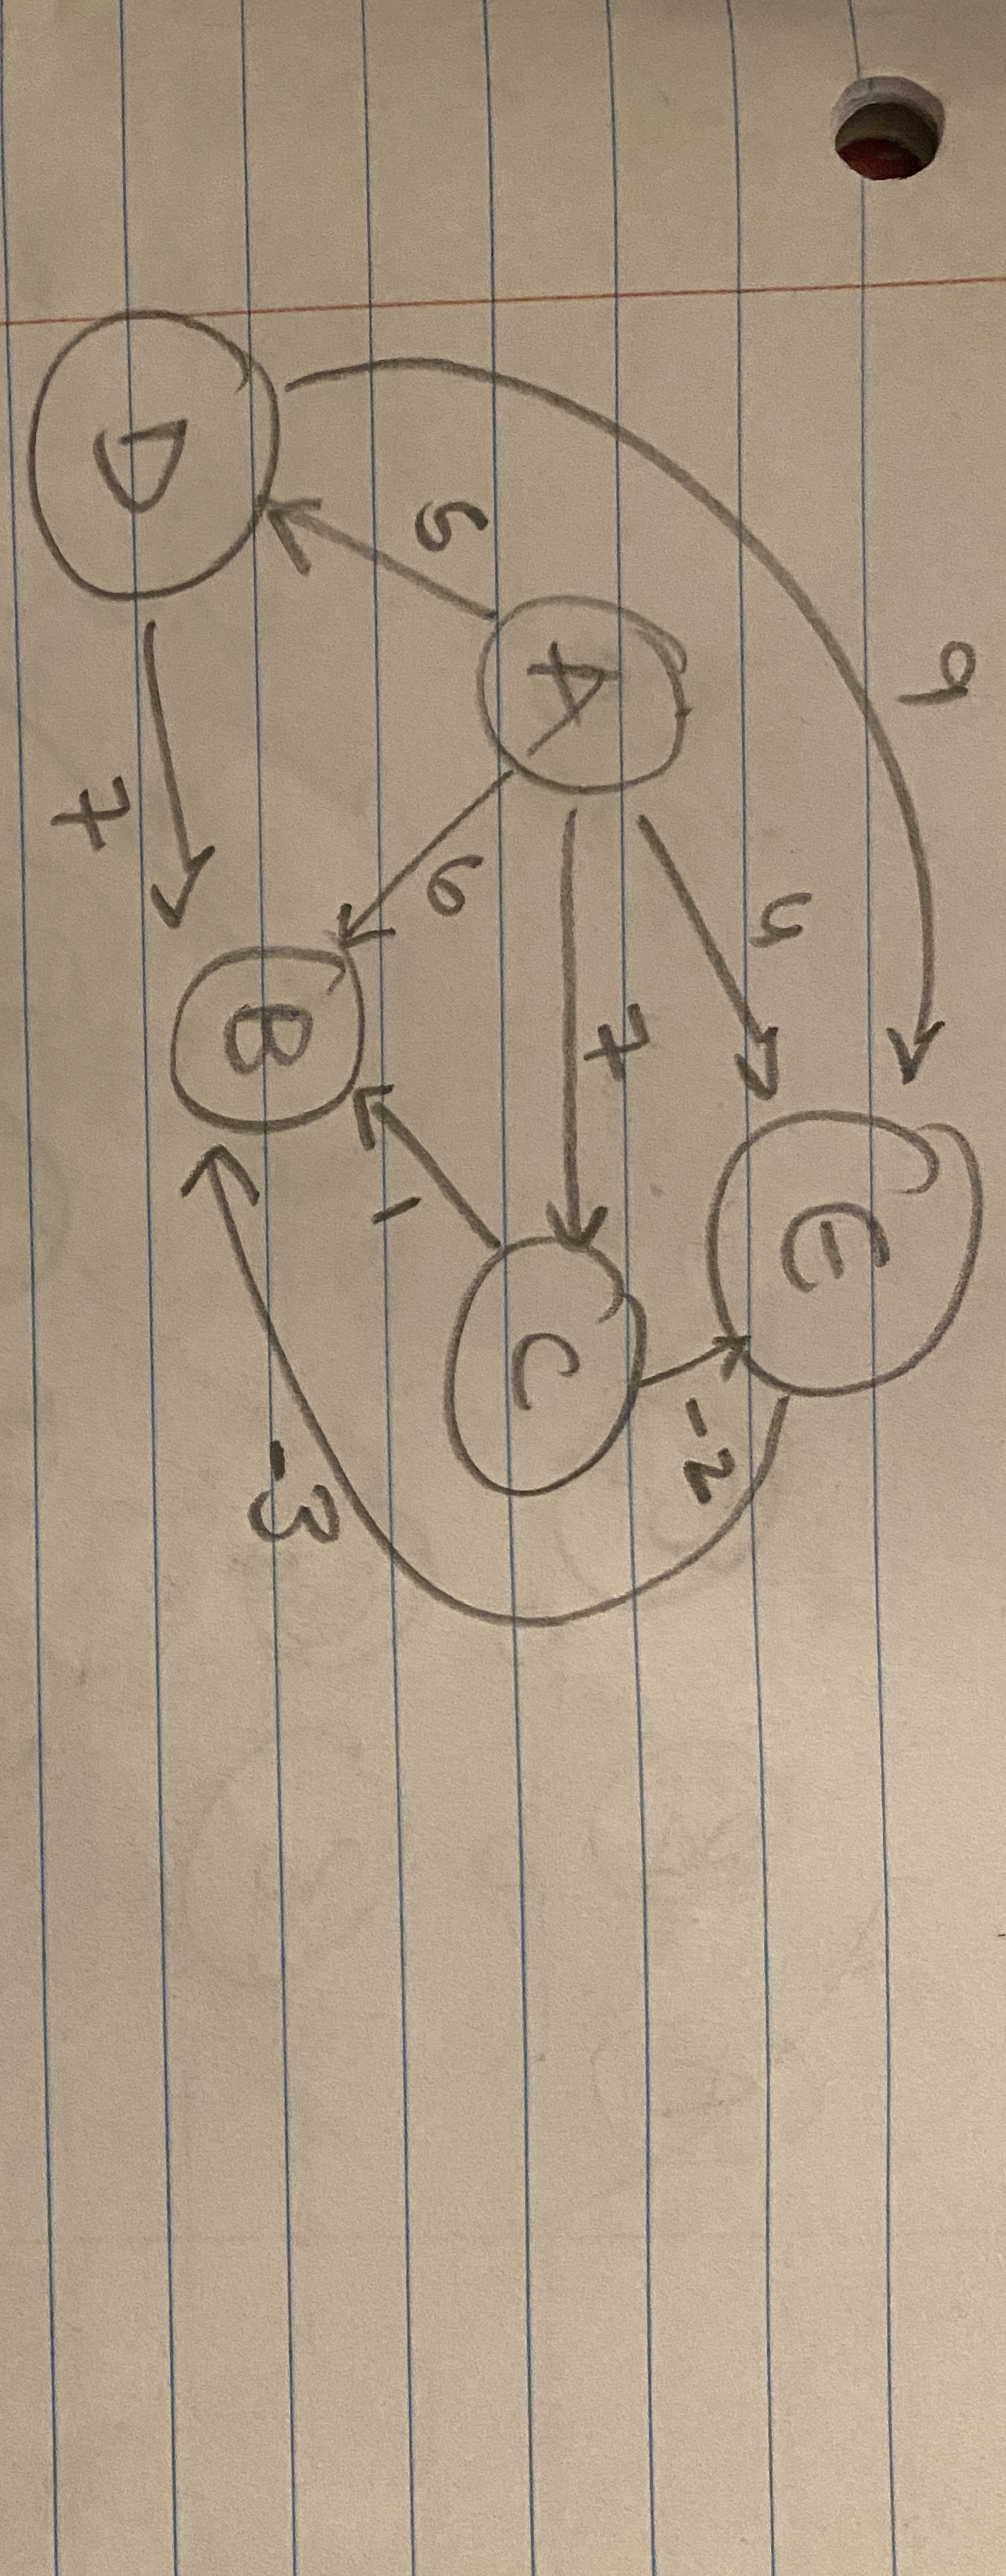
\includegraphics[scale=0.1,angle=90]{IMG_8569.JPG}
\end{enumerate}

\pagebreak

\item Problem 5. Exercise 26.1-7 (page 714).\\
On modeling vertex capacity constraints. Include a drawing, showing how a vertex v in G (with limit l(v) and some in-edges and some out-edges) is represented in G'. Also, what are the source and sink in G'?\\

Exercise 26.1-7 (page 714):
Suppose that, in addition to edge capacities, a flow network has \textbf{vertex capacities}. That is each vertex \textit{v} has a limit l(v) on how much flow can pass though v. Show how to transform a flow network G = (V,E) with vertex capacities into an equivalent flow network G' = (V', E') without vertex capacities, such that a maximum flow in G' has the same value as a maximum flow in G. How many vertices and edges does G' have?
\begin{enumerate}
    \item Let us begin by thinking about how the network flow G' will operate. It will be a network between two vertices $v_1$ and $v_2$ which have the aforementioned limit of l(v) and this will ascertain the flow on G'. 
    \item The two vertices $v_1$ and $v_2$ will be formed by splitting an existing vertex v which initially was a part of the network flow G. So all the inlet edges of the network flow that were coming to v will now be channeled towards vertex $v_1$. The same thing will apply for vertex $v_2$ - all the outlet edges of the network flow that were leaving from v will now leave from vertex $v_2$.
    \item Now let us determine functions which will help us solve this problem. We will need a function for the network flow on G and G' respectively. On network flow G, we will call this function f. On network flow G', we our flow function will be referred to as f' and will be based on (following notation seen on pg 709):
    \begin{enumerate}
        \item For each edge (u, v) in the network flow G, $f'(u_2, v_1) = f(u, v)$
        \item For each vertex u which belongs to the set of vertices V, let $f'(u_1, u_2) = $ the sum of all $f(u, v)$ for every v in V.
        \item $f'(t_1, t_2) = $ the sum of all $f(v, t)$ for every v in V. t is part of V, V goes up till t (where t is the target vertex, and s is the source vertex)
    \end{enumerate}
    \item Through the above, a one-to-one relationship is identified amongst the networks which follow the flow limit of l(v) in G', and those which follow the capacities of the vertices in G. 
    \item Looking at all the edges: any edge of the form $(u_1, u_2)$ is part of E'. E' essentially contains all the edges in E (edges which help create network flow G) of the form $(u, v)$. \\
    For the edges in E', we see that they mimic the constraints observed in E, which are constrained by the vertex capacities in G. Given this, we obtain an understanding that:
    \begin{enumerate}
        \item $f'(u_1, u_2) = $ the sum of all $f(u, v) \leq l(u) = c'(u_1, u_2)$ for every v in V \\the above exists for every $u$ which belongs to $V = {s,t}$
        \item We also need a constraint imposing the capacities on vertex which form G. This is given by:  $f'(t_1, t_2+ = $ the sum of all $f(v,t) \leq l(t) = c'(t_1, t_2)$ for every v in V\\ 
        Please note, the references to l() refer to: an edge $(v_1, v_2)$ in E' with $c(v_1, v_2) = l(v)$ (where c() refers to capacity constraints)
    \end{enumerate}
    \item After building the groundwork required for the understanding of this problem, we can now look at the meat of solving this sum. This involves proving that the flow is conserved throughout the creation of the equivalent network flow G'.
    \item Looking at all vertices u which are in V {s,t}, we verify flow conservation as follows:
    \begin{enumerate}
        \item Summation of each of the following lines\\
        incoming flow to $t_1$ is: 
        \begin{enumerate}
            \item $f'(v, t_1)$ (for all values v which belong to V')
            \item $f(v, t)$ (for all values v which belong to V)
            \item $f'(t_1, t_2)$ (for all values v which belong to V; to maintain flow of conservation law)
            \\Since we observe that the incoming flow to $t_1$ is equal to the outgoing flow from to $t_1$, flow conservation is conserved. Let us look at other parts now, first let us see if flow was conserved at $u_1$.
        \end{enumerate}
    \end{enumerate}
    
    \begin{enumerate}
        \item Summation of each of the following lines\\
        incoming flow to $u_1$ is: 
        \begin{enumerate}
            \item $f'(v, u_1)$ (for all values v which belong to V')
            \item $f(v, u)$ (for all values v which belong to V)
            \item $f(u, v)$ (for all values v which belong to V; to maintain flow of conservation law)
            \item $f'(u_1, u_2)$ \\Since we observe that the incoming flow to $u_1$ is equal to the outgoing flow from to $u_1$, flow conservation is conserved. Let us look at other parts now, namely $u_2$
        \end{enumerate}
    \end{enumerate}
    
    \begin{enumerate}
        \item Summation of each of the following lines\\
        For any edge $u_2 != t_2$ (they are not equal): 
        \begin{enumerate}
            \item $f'(u_1, u_2)$ (no summation; this is the incoming flow)
            \item $f(u, v)$ (for all values v which belong to V)
            \item $f'(u_2, v)$ (for all values v which belong to V')\\Since we observe that the incoming flow is equal to the outgoing flow, flow conservation is conserved.
        \end{enumerate}
    \end{enumerate}
    \item Given the above, we were able to prove that our thoughts about the solution to this question are correct (and hence our calculations for the vertices and edges in G’) because of the principle of flow conservation being maintained. 
\end{enumerate}
\begin{enumerate}
    \item \textbf{Condensed Explanation:}\\
    Each vertex is split. The limit of the original vertex becomes the weight of edge between the two vertices (which were formed after splitting). \\
    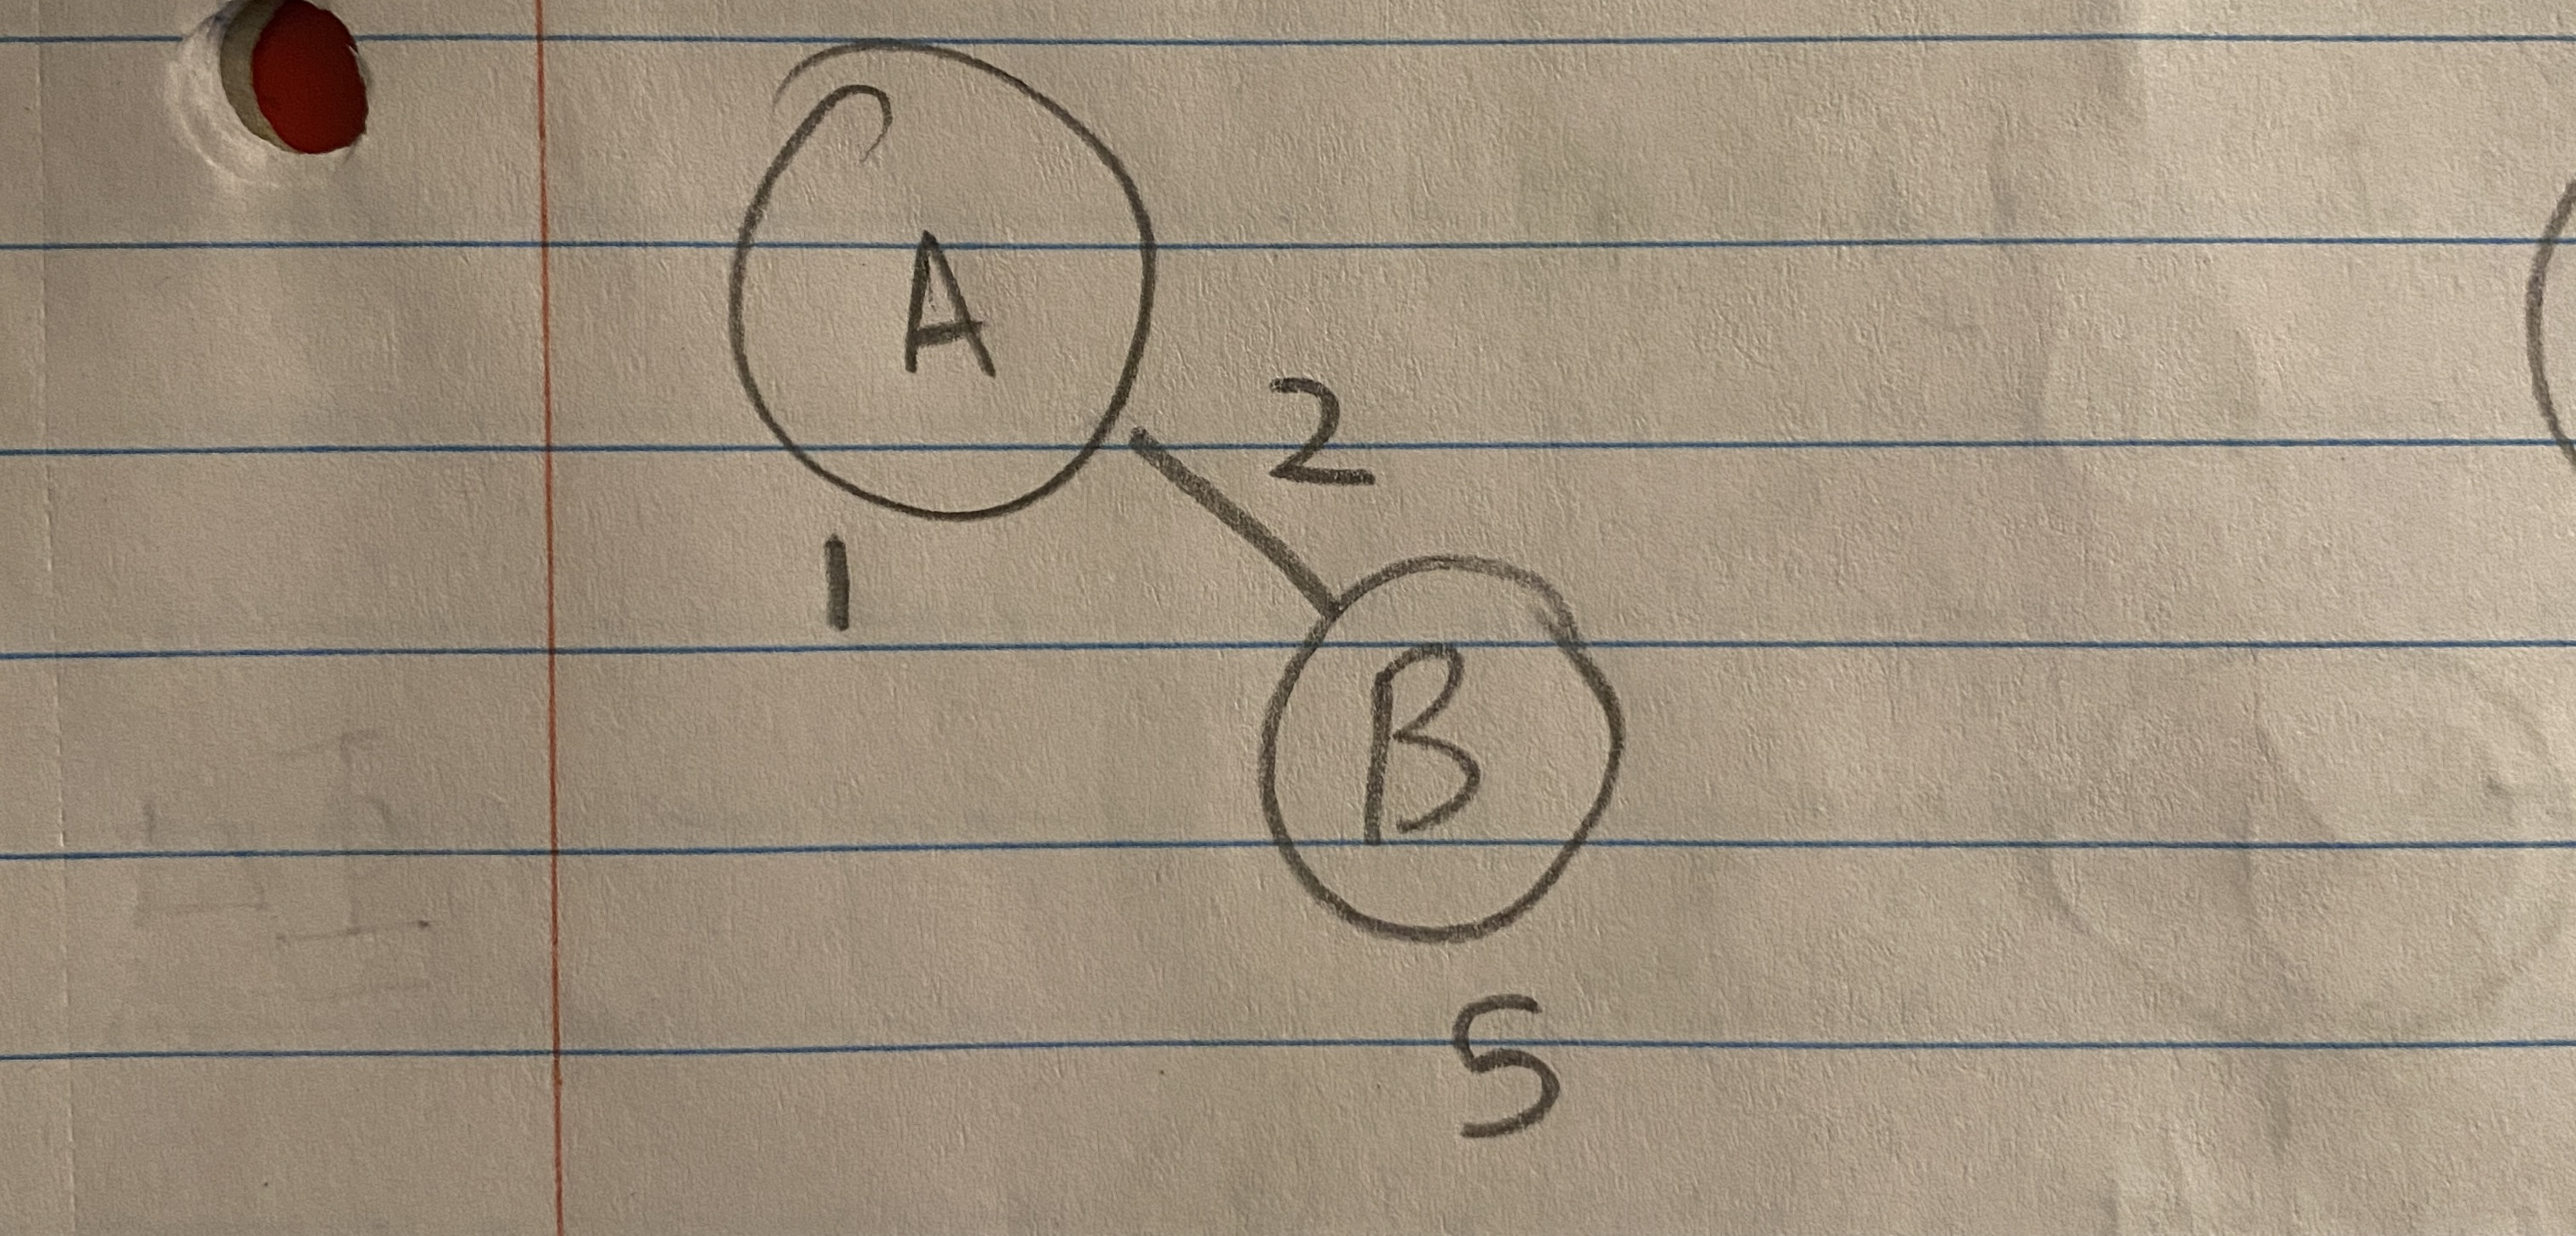
\includegraphics[scale=0.1]{IMG_8564.JPG}
    \item Edges going from A to B become A to B1. If there was an outgoing edge from node B in the original graph, then we would have to add an outgoing edge from B2 to the next vertex. This would effectively void the limit on vertex B. Since this is beneficial, a similar operation is performed on all the vertices.\\
    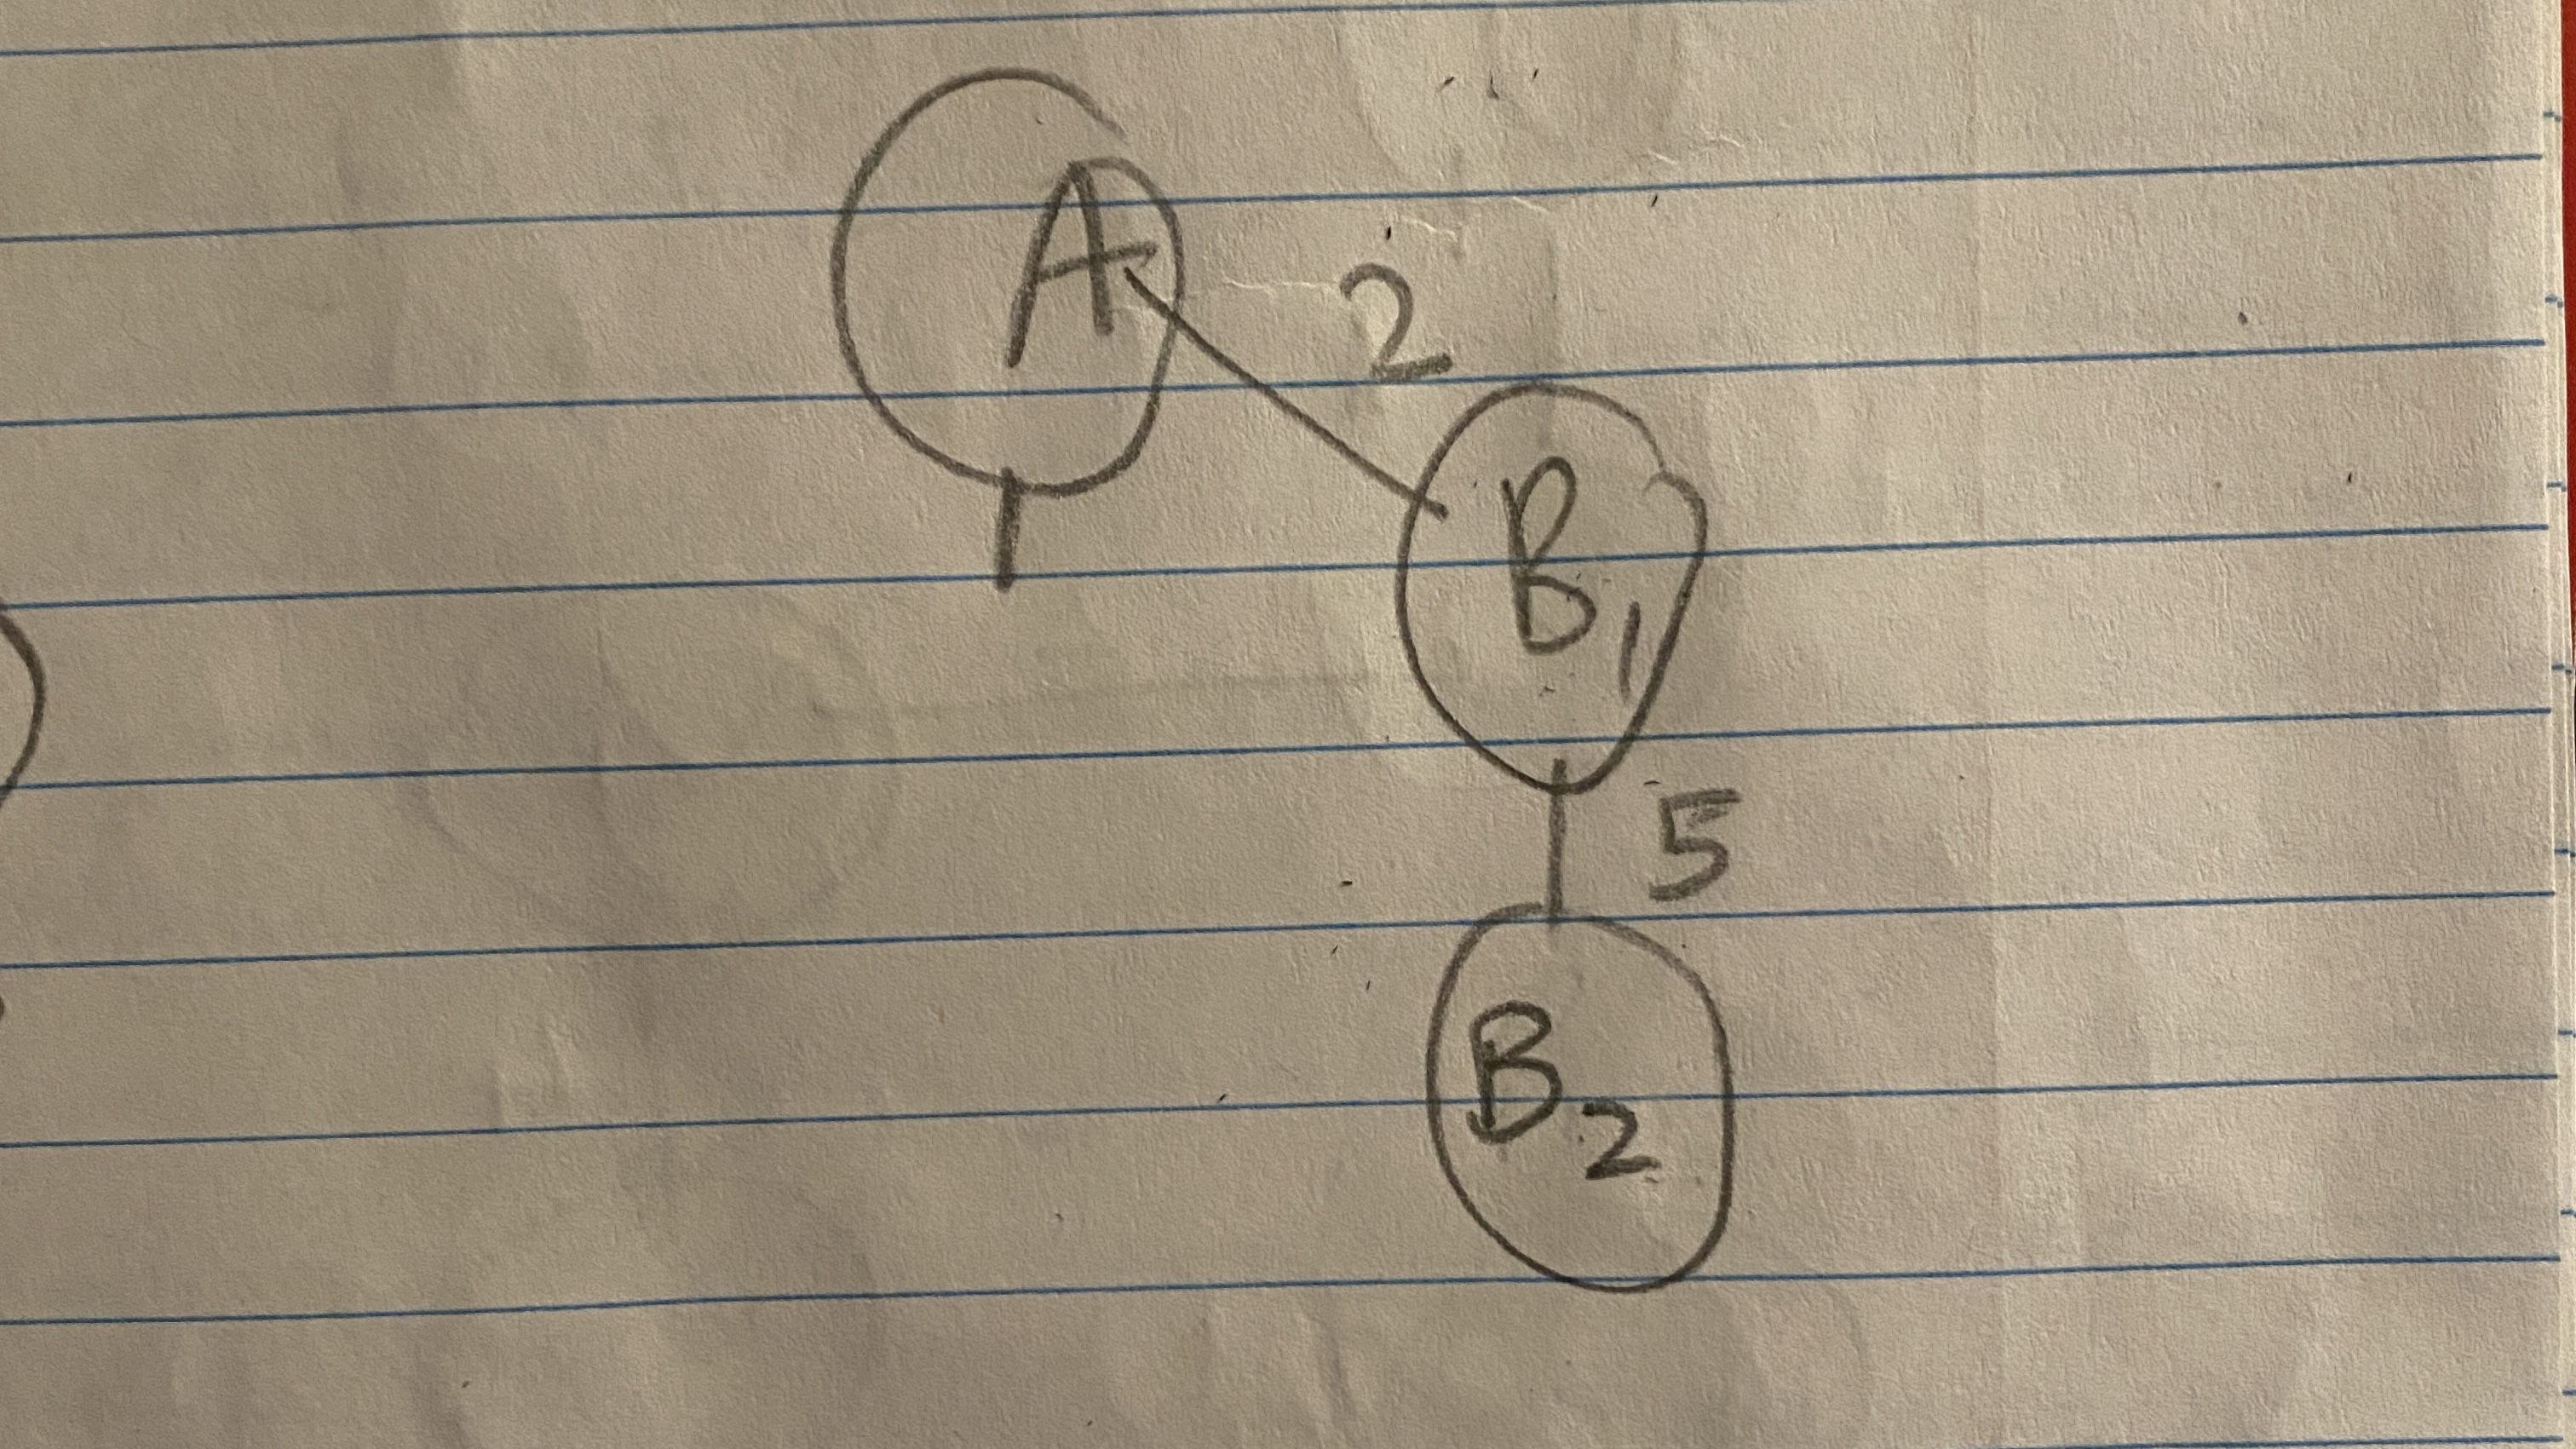
\includegraphics[scale=0.1]{IMG_8566.JPG}
    \item Using this (and as seen in the diagram), we can conclude that the Maxflow doesn't change because the flow is conserved (outgoing and incoming are equal).\\
    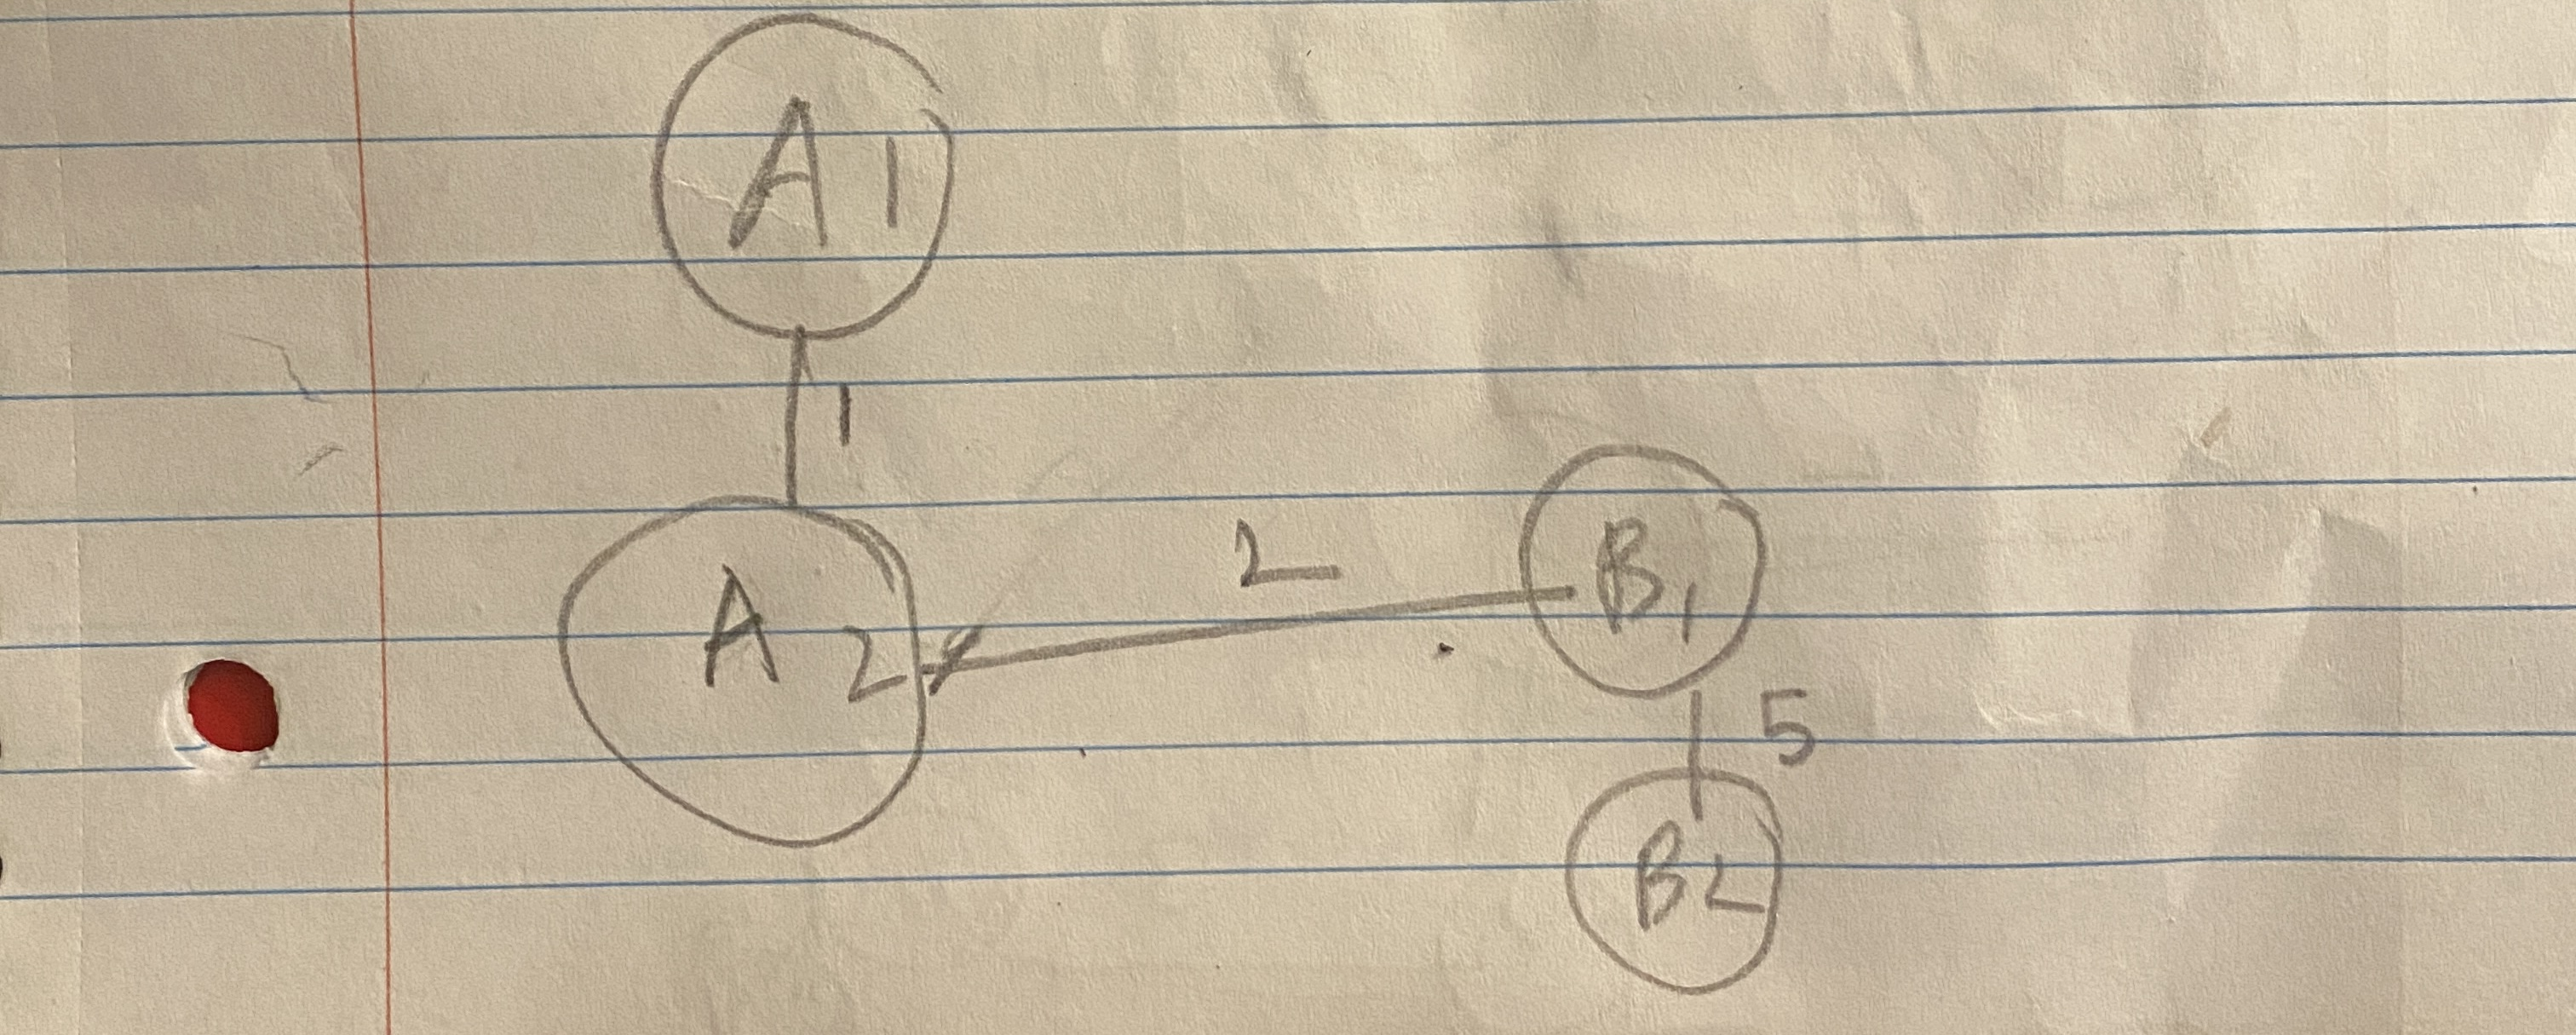
\includegraphics[scale=0.1]{IMG_8567.JPG}
\end{enumerate}
\pagebreak

\end{enumerate}

\end{document}

$f'(t_1, t_2)$